%% %%%%%%%%%%%%%%%%%%%%%%%%%%%%%%%%%%%%%%%%%%%%%%%%
%% Problem Set/Assignment Template to be used by the
%% Food and Resource Economics Department - IFAS
%% University of Florida's graduates.
%% %%%%%%%%%%%%%%%%%%%%%%%%%%%%%%%%%%%%%%%%%%%%%%%%
%% Version 1.0 - November 2019
%% %%%%%%%%%%%%%%%%%%%%%%%%%%%%%%%%%%%%%%%%%%%%%%%%
%% Ariel Soto-Caro
%%  - asotocaro@ufl.edu
%%  - arielsotocaro@gmail.com
%% %%%%%%%%%%%%%%%%%%%%%%%%%%%%%%%%%%%%%%%%%%%%%%%%

\documentclass[11pt]{article}
\usepackage{float}
\usepackage[ruled,vlined,linesnumbered,algo2e]{algorithm2e}
\usepackage{algorithm}
\usepackage{amsmath,amssymb}
\usepackage{amsthm}
\usepackage{makecell}
\usepackage{tikz}
\usepackage[a4paper, total={6.5in, 9in}]{geometry}
\usepackage[style=authoryear, backend=biber]{biblatex}
\bibliography{bibliography.bib}
\newcommand*\circled[1]{\tikz[baseline=(char.base)]{
   \node[shape=circle,draw=red,inner sep=1pt] (char) {#1};}}
\setlength\parindent{0pt} %% Do not touch this
\DeclareMathOperator{\phiAb}{\phi_{\mathbf{A},\mathbf{b}}}
\DeclareMathOperator{\spn}{span}
\newtheorem{lemma}{Lemma}
\newtheorem{theorem}{Theorem}
\newtheorem{definition}{Definition}
\newtheorem{corollary}{Corollary}[theorem]

\usepackage{pgfplots}
\pgfplotsset{compat=newest}
  %% the following commands are needed for some matlab2tikz features
\usetikzlibrary{plotmarks}
\usetikzlibrary{arrows.meta}
\usepgfplotslibrary{patchplots}
\usepackage{grffile}
\usepackage{amsmath}
\usepackage{subcaption}

\usepgfplotslibrary{external} 
\tikzexternalize


\numberwithin{equation}{section}

%% -----------------------------
%% TITLE
%% -----------------------------
\title{Note on Matrix functions} %% Assignment Title
\author{Nathan Rousselot}
%% Change "\today" by another date manually
%% -----------------------------
%% -----------------------------

%% %%%%%%%%%%%%%%%%%%%%%%%%%
\begin{document}
%\setlength{\droptitle}{-5em}    
%% %%%%%%%%%%%%%%%%%%%%%%%%%
\maketitle

\section{Introduction}
In this document we introduce the notion of matrix functions. Say we have a function $f:\mathbb{C}\rightarrow\mathbb{C}$, then we can define the function $f$ on a matrix $\mathbf{A}$ as follows: $f:\mathbb{C}^{n\times n}\rightarrow\mathbb{C}^{n\times n}$. In the following, we will first provide some theoretical background on matrix functions. Then, we will describe the numerical issues coming with manipulating matrix functions. Finally, we will provide algorithm for efficient computation of matrix fuctions.

\section{Theoretical background}
\subsection{Natural Definition}
\subsubsection*{Polynomial functions}
Let $p:\mathbb{C}\rightarrow\mathbb{C}$ be a polynomial function of degree $d$:
\begin{equation}
    p(t) = \sum_{k=0}^d c_k t^k
\end{equation}
Then, considering a matrix $\mathbf{A}\in\mathbb{C}^{n\times n}$, and posing $\mathbf{A}^0 = I_n$, we can define the polynomial function $p:\mathbb{C}^{n\times n}\rightarrow\mathbb{C}^{n\times n}$ on a matrix $\mathbf{A}$ as follows:
\begin{equation}
    p(\mathbf{A}) = \sum_{k=0}^d c_k \mathbf{A}^k
\end{equation}

\subsubsection*{Rational functions}
Let $f:\mathbb{C}\rightarrow\mathbb{C}$ be a rational function of the form:
\begin{equation}
    f(t) := \frac{p(t)}{q(t)}
\end{equation}
It is not immediate how one would approach this function with a matrix. We want to define
\begin{equation}\label{eq:rationale}
    f(\mathbf{A}) := q(\mathbf{A})^{-1}p(\mathbf{A})
\end{equation}
However, this is not well defined if $q(\mathbf{A})$ is singular. In other words, we need to make sure that $q(\mathbf{A})$ is invertible. This is the case if and only if $q(\lambda) \neq 0$ for all eigenvalues $\lambda$ of $\mathbf{A}$. This is a very strong condition, and it is not always possible to find a rational function $f$ such that $q(\lambda) \neq 0$ for all eigenvalues $\lambda$ of $\mathbf{A}$. We note that a choice in notation has been made in equation \ref{eq:rationale}, the other notation is still valid.
\begin{lemma}\label{lem:commute}
     Let $\mathbf{A}\in\mathbb{C}^{n\times n}$, and let $p:\mathbb{C}^{n\times n}\rightarrow\mathbb{C}^{n\times n}$ and $q:\mathbb{C}^{n\times n}\rightarrow\mathbb{C}^{n\times n}$, two matrix polynomials. Then,
     \begin{equation}
         q(\mathbf{A})p(\mathbf{A}) = p(\mathbf{A})q(\mathbf{A})
     \end{equation}
\end{lemma}
\begin{proof}
    Let $f(\mathbf{A}) := q(\mathbf{A})p(\mathbf{A})$, and $g(\mathbf{A}) = p(\mathbf{A})q(\mathbf{A})$. Then
    \begin{align*}
        f(\mathbf{A}) = \left(\sum_{k=0}^d c_k\mathbf{A}^k\right)\left(\sum_{j=0}^m b_j\mathbf{A}^j\right)\\
        = \sum_{k=0}^d \sum_{j=0}^m c_kb_j\mathbf{A}^{j+k}\\
        = \sum_{j=0}^m \sum_{k=0}^d b_jc_k\mathbf{A}^{k+j}\\
        = \left(\sum_{j=0}^m b_j\mathbf{A}^j\right)\left(\sum_{k=0}^d c_k\mathbf{A}^k\right) = g(\mathbf{A})
    \end{align*}
\end{proof}
\begin{theorem}
    Let $\mathbf{A}\in\mathbb{C}^{n\times n}$, and let $p:\mathbb{C}^{n\times n}\rightarrow\mathbb{C}^{n\times n}$ and $q:\mathbb{C}^{n\times n}\rightarrow\mathbb{C}^{n\times n}$, two matrix polynomials such that $q(\mathbf{A})$ is non-singular. Then, 
    \begin{equation}
        q(\mathbf{A})^{-1}p(\mathbf{A}) = p(\mathbf{A})q(\mathbf{A})^{-1}
    \end{equation}
\end{theorem}
\begin{proof}
    Let $\mathbf{A}\in\mathbb{C}^{n\times n}$ be a matrix such that $q(\mathbf{A})$ is non-singular
    \begin{align*}
        q(\mathbf{A})^{-1}p(\mathbf{A}) = q(\mathbf{A})^{-1}p(\mathbf{A})q(\mathbf{A})q(\mathbf{A})^{-1} 
    \end{align*}
    Using Lemma \ref{lem:commute}
    \begin{align*}        
    q(\mathbf{A})^{-1}p(\mathbf{A})q(\mathbf{A})q(\mathbf{A})^{-1} = q(\mathbf{A})^{-1}q(\mathbf{A})p(\mathbf{A})q(\mathbf{A})^{-1} \\
        = p(\mathbf{A})q(\mathbf{A})^{-1}
    \end{align*}
\end{proof}

\subsubsection*{Power Series}
Let $f:\mathbb{C}\rightarrow\mathbb{C}$ be a function that can be expressed as a power series:
\begin{equation}
    f(t) = \sum_{k=0}^\infty c_k t^k
\end{equation}
Then, considering a matrix $\mathbf{A}\in\mathbb{C}^{n\times n}$, and posing $\mathbf{A}^0 = I_n$, we can define the power series function $f:\mathbb{C}^{n\times n}\rightarrow\mathbb{C}^{n\times n}$ on a matrix $\mathbf{A}$ as follows:
\begin{equation}
    f(\mathbf{A}) = \sum_{k=0}^\infty c_k \mathbf{A}^k
\end{equation}
In the scalar case, we know that the power series converges if $|t| < r$, where $r$ is the radius of convergence. Obviously this translates in the matrix power series
\begin{theorem}\label{th:power_convergence}
    Let $f:\mathbb{C}^{n\times n}\rightarrow\mathbb{C}^{n\times n}$ be a matrix power series. Then, the series converges if and only if $\rho(\mathbf{A}) < r$, where $\rho(\mathbf{A})$ is the spectral radius of $\mathbf{A}$, and $r$ is the radius of convergence of the scalar power series.
\end{theorem}
Proof is provided in \cite{frommer2008matrix}. In the case of a finite-order Laurent Series, \textit{i.e}:
\begin{equation}
    f(t) = \sum_{k=-d}^d c_k t^k
\end{equation}
For the matrix case, we need to ensure convergence (similarly to power series), but also ensure existance of the inverse, as Laurent series do have negative powers. If both of those conditions are satisfied, we can write the Laurent series as a matrix function:
\begin{equation}
    f(\mathbf{A}) = \sum_{k=-d}^d c_k \mathbf{A}^k
\end{equation}
\subsection{Spectrum-Based Definition}
\subsubsection*{Diagonalizable Matrices}
Let $\mathbf{A}\in\mathbb{C}^{n\times n}$ be a diagonalizable matrix. That means that there exists a matrix $\mathbf{V}\in\mathbb{C}^{n\times n}$ such that $\mathbf{V}$ is invertible, and $\mathbf{A} = \mathbf{V}\mathbf{\Lambda}\mathbf{V}^{-1}$, where $\mathbf{\Lambda}$ is a diagonal matrix containing the eigenvalues of $\mathbf{A}$ :
\begin{equation}
    \mathbf{\Lambda} = \begin{bmatrix}
        \lambda_1 & 0 & \cdots & 0 \\
        0 & \lambda_2 & \cdots & 0 \\
        \vdots & \vdots & \ddots & \vdots \\
        0 & 0 & \cdots & \lambda_n
    \end{bmatrix}
\end{equation}
\begin{theorem}
    Let $\mathbf{A}\in\mathbb{C}^{n\times n}$ be a diagonalizable matrix. Then we can define the function $f(\mathbf{A})$ as:
    \begin{equation}
        f(\mathbf{A}) := \mathbf{V}f(\mathbf{\Lambda})\mathbf{V}^{-1}
    \end{equation}
    with 
    \begin{equation}
        f(\mathbf{\Lambda}) = \begin{bmatrix}
            f(\lambda_1) & 0 & \cdots & 0 \\
            0 & f(\lambda_2) & \cdots & 0 \\
            \vdots & \vdots & \ddots & \vdots \\
            0 & 0 & \cdots & f(\lambda_n)
        \end{bmatrix}
    \end{equation}        
\end{theorem}
This property is very handy, as it allows us to compute matrix functions by simply applying the function to the eigenvalues of the matrix. Computationally, this avoids inverting matrices, and lots of matrix products. However, this property is only valid for diagonalizable matrices. This property puts constraints on $f(\mathbf{A})$, as its eigenvectors must form a basis $\mathbf{F}^n$. Another more practical constraint, that is sufficient but not necessary, is if $\mathbf{A}$ is a full rank matrix, then it is diagonalizable.

\subsubsection*{Defective Matrices}
In some cases, the matrix $\mathbf{A}$ is not diagonalizable, that means the sum of the dimensions of the eigenspaces is less than $n$, we call that a \textit{Defective Matrix}. In that case, we can generalize the principle of diagonalization using the Jordan canonical form of $\mathbf{A}$:
\begin{equation}
    \mathbf{A} = \mathbf{V}\mathbf{J}\mathbf{V}^{-1}
\end{equation}
where $\mathbf{J}$ is a Jordan matrix, and $\mathbf{V}$ is a matrix containing the generalized eigenvectors of $\mathbf{A}$. The Jordan matrix is a block diagonal matrix, where each block is a Jordan block. A Jordan block is a matrix of the form:
\begin{equation}
    \mathbf{J}_k(\lambda) = \begin{bmatrix}
        \lambda & 1 & 0 & \cdots & 0 \\
        0 & \lambda & 1 & \cdots & 0 \\
        \vdots & \vdots & \ddots & \ddots & \vdots \\
        0 & 0 & \cdots & \lambda & 1 \\
        0 & 0 & \cdots & 0 & \lambda
    \end{bmatrix}
\end{equation}
\begin{theorem}\label{thm:jordan}
    Let $\mathbf{A}\in\mathbb{C}^{n\times n}$ be a defective matrix. Then we can define the function $f(\mathbf{A})$ as:
    \begin{equation}
        f(\mathbf{A}) := \mathbf{V}f(\mathbf{J})\mathbf{V}^{-1}
    \end{equation}
    with 
    \begin{equation}
        f(\mathbf{J}) = \begin{bmatrix}
            f(\mathbf{J}_1(\lambda_1)) & 0 & \cdots & 0 \\
            0 & f(\mathbf{J}_2(\lambda_2)) & \cdots & 0 \\
            \vdots & \vdots & \ddots & \vdots \\
            0 & 0 & \cdots & f(\mathbf{J}_k(\lambda_k))
        \end{bmatrix}
    \end{equation}
    and \begin{equation}
        f(\mathbf{J}_i(\lambda_i)) = \begin{bmatrix}
            f(\lambda_i) & f'(\lambda_i) & \frac{f''(\lambda_i)}{2!} & \cdots & \frac{f^{(k-1)}(\lambda_i)}{(k-1)!} \\
            0 & f(\lambda_i) & f'(\lambda_i) & \cdots & \frac{f^{(k-2)}(\lambda_i)}{(k-2)!} \\
            \vdots & \vdots & \ddots & \ddots & \vdots \\
            0 & 0 & \cdots & f(\lambda_i) & f'(\lambda_i) \\
            0 & 0 & \cdots & 0 & f(\lambda_i)
        \end{bmatrix}
    \end{equation}
\end{theorem}
Obviously, both definitions of matrix functions, based on diagonalization and Jordan canonical form, presuppose that the spectral radius of $\mathbf{A}$, $\rho(\mathbf{A})$, is less than $r$, the radius of convergence.
\subsection{Interpolation-based definition}
Interestingly, in this section we will show that for any $\mathbf{A}\in\mathbb{C}^{n\times n}$ and any sufficiently differentiable $f$, we can find a polynomial $p$ such that $f(\mathbf{A})=p(\mathbf{A})$. First, let us observe from previous sections that only the eigenvalues of $\mathbf{A}$ are actually important for matrix polynomials. Also recall that every matrix $\mathbf{A}\in\mathbb{C}^{n\times n}$ with spectrum $\{\lambda_1,\dots,\lambda_n\}$ has a minimal polynomial $\phi_{\mathbf{A}}$ given by
\begin{equation}\label{eq:minimalpoly}
\phi_{\mathbf{A}}(t):=\prod_{i=1}^{k}(t-\lambda_k)^{n_i}
\end{equation}
which is the unique monic minimal degree ($\text{degr}(\phi_{\mathbf{A}})=n_1+\cdots+n_k\leq n$) polynomial such that $\phi_{\mathbf{A}}(\mathbf{A})=0$.
\begin{theorem}\label{thm:unicity}
Let $\mathbf{A}\in \mathbb{C}^{n\times n}$ be a matrix with eigenvalues $\{\lambda_1,\ldots,\lambda_k\}$, and minimal polynomial given by equation~\ref{eq:minimalpoly}. Then for any two polynomials $p_1,p_2$ we have that $p_1(\mathbf{A})=p_2(\mathbf{A})$ if and only if 
$$\forall j\in\{1,\ldots,k\}:\forall i\in\{0,\ldots,n_k-1\}: p_1^{(i)}(\lambda_j)=p_2^{(i)}(\lambda_j).$$
\end{theorem}
\begin{proof}
    Let $\mathbf{A}\in\mathbb{C}^{n\times n}$, with spectrum $\{\lambda_1,\ldots,\lambda_k\}$, and two polynomials $p_1$ and $p_2$ such that $p_1(\mathbf{A})=p_2(\mathbf{A})$. Let us define $q$ such that
    \begin{equation*}
        q := p_1 - p_2
    \end{equation*}
    Then, $q(\mathbf{A})=0$, and is thus divisible by $\phi_{\mathbf{A}}$, meaning that
    \begin{equation*}
        \forall j\in\{1,\dots,k\}:\forall i\in\{0,\ldots,n_k-1\}, q(\lambda_j) = 0 \Rightarrow p_1^{(i)}(\lambda_j) = p_1^{(i)}(\lambda_i)
    \end{equation*}
    Similarly, consider two polynomials $p_1$ and $p_2$ such that 
    \begin{equation*}
        \forall j\in\{1,\dots,k\}:\forall i\in\{0,\ldots,n_k-1\},  p_1^{(i)}(\lambda_j) = p_2^{(i)}(\lambda_i)    
    \end{equation*}
    For $i=0$, $q:=p_1-p_2=0$ on the spectrum of $\mathbf{A}$, and is then divisible by $\phi_{\mathbf{A}}$. Then
    \begin{equation*}
        q = K\phi_{\mathbf{A}}
    \end{equation*}
    with $K$ a polynomial. Then, $q(\mathbf{A})=K(\mathbf{A})\phi_{\mathbf{A}}(\mathbf{A}) = 0$ since by definition, $\phi_{\mathbf{A}}(\mathbf{A}) = 0$. And thus, $p_1(\mathbf{A})=p_2(\mathbf{A})$.

    From this reasoning, we conclude that 
    \begin{align*}
        p_1(\mathbf{A}) = p_2(\mathbf{A}) \\ \Leftrightarrow \forall j\in\{1,\ldots,k\}:\forall i\in\{0,\ldots,n_k-1\}: p_1^{(i)}(\lambda_j)=p_2^{(i)}(\lambda_j)
    \end{align*}
\end{proof}
In theorem~\ref{thm:unicity}, the conditions involve the evaluation of the polynomials $p_1$ and $p_2$ and their derivatives up to order $n_k-1$ at the eigenvalues of $A$.

However, when the spectrum of $A$ is simple, each eigenvalue $\lambda_j$ is of multiplicity $n_j=1$. This means that there are no higher order terms corresponding to these eigenvalues in the minimal polynomial, or in other words, there are no repeated roots. Consequently, there is no need to consider the derivatives of the polynomials $p_1$ and $p_2$ because there are no repeated roots for the polynomials to ``match up'' with. Therefore, in this simpler case, we only need to check that the polynomials $p_1$ and $p_2$ agree at the eigenvalues of $A$. In formal terms, the condition becomes:
\begin{corollary}\label{cor:unicity}
Let $\mathbf{A}\in \mathbb{C}^{n\times n}$ be a matrix with eigenvalues $\{\lambda_1,\ldots,\lambda_k\}$, and minimal polynomial given by equation~\ref{eq:minimalpoly}. If $\mathbf{A}$ has simple spectrum, then for any two polynomials $p_1,p_2$ we have that $p_1(\mathbf{A})=p_2(\mathbf{A})$ if and only if
\begin{equation*}
    \forall j\in\{1,\ldots,k\}: p_1(\lambda_j)=p_2(\lambda_j).
\end{equation*}
\end{corollary}
From this corollary, and from theorem \ref{thm:unicity}, we can confirm our earlier statement : only the spectrum of $\mathbf{A}$ is important for matrix polynomials. More importantly, we observe that $p(\mathbf{A})$ is uniquely defined by its values on the spectrum of $\mathbf{A}$. It seems then natural to extend this definition to any function $f$.
\begin{definition}\label{def:Hermite}
    Let $\mathbf{A}\in\mathbb{C}^{n\times n}$ be a matrix with minimal polynomial given as in equation \ref{eq:minimalpoly}, and let $f$ be a function that is at least $\max_k\{n_k-1\}$ times differentiable. Say $p$ is its $(n_1,\ldots,n_k)$-\emph{Hermite interpolant} i.e. the polynomial satisfying
    $$\forall j\in\{1,\ldots,k\}:\forall i\in\{0,\ldots,n_k-1\}: p^{(i)}(\lambda_j)=f^{(i)}(\lambda_j)$$
    of minimal degree. Then we define $f(\mathbf{A})=p(\mathbf{A})$.
\end{definition}
%%%%%%% NEED TO COMMENT ON THIS %%%%%%%%
\section{The matrix-vector product $f(\mathbf{A})\mathbf{b}$}
\subsection{Introduction}\label{sec:fabintro}
To motivate the need for a matrix-vector product, we will consider a matrix $\mathbf{A}\in\mathbb{C}^{n\times n}$. Let us consider the matrix exponential, such as :
\begin{equation}
    e^{\mathbf{A}} = \sum_{k=0}^\infty \frac{\mathbf{A}^k}{k!}
\end{equation}
Not only does this computation is very heavy (see section \ref{sec:matrixexp} for computation strategies), but it also affects the structure of the matrix. Say for example, we have the following laplacian matrix: 
\begin{equation*}
    \mathbf{A} = \begin{bmatrix}
        2 & -1 & 0 & 0 & \dots &  \dots & 0 \\
        -1 & 2 & -1 & 0 & 0 & \dots & 0 \\
        0 & -1 & 2 & -1 & 0 & \dots & 0 \\
        \vdots & \vdots & \ddots & \ddots & \ddots & \ddots & \vdots \\
        0 & 0 & \dots & 0 & -1 & 2 & -1 \\
        0 & 0 & \dots & 0 & 0 & -1 & 2
    \end{bmatrix}
\end{equation*}
Obviously, $\mathbf{A}$ is a sparse matrix, and also a rank-structured one : it is a tridiagonal matrix. However, by computing $e^{\mathbf{A}}$, one will get a dense matrix. Storing a dense matrix often becomes challenging as the dimension of the problem grows. Besides storing, computing such a dense matrix is also an issue. However, the matrix-vector product $f(\mathbf{A})\mathbf{b}$ can be stored and computed efficiently.

\subsection{The Method}
As motivated by \ref{sec:fabintro}, when encountering specific structure in $\mathbf{A}$, such as sparsity, there is a lot to gain if we can store $f(\mathbf{A})\mathbf{b}$. In this section we will work towards a way to evaluate $f(\mathbf{A})\mathbf{b}$ in an intuitive way, thanks to Arnoldi method.

\subsubsection{Formal Definitions}
Firstly, we will define the notion of $\phiAb$, i.e. the minimal polynomial of $\mathbf{A}$ with respect to the vector $\mathbf{b}$. This is simply the polynomial
\begin{equation}\label{eq:minPolyAb}
\phiAb(t):= \prod_{i=1}^{k}(t-\lambda_i)^{m_i}
\end{equation}
of minimal degree such that $\phiAb(\mathbf{A})\mathbf{b}=\mathbf{0}$. Here $\lambda_1,\ldots,\lambda_k$ are again the eigenvalues of $\mathbf{A}$.

%%%%% EXAMPLE WHERE PHIab =/= PHIa %%%%%

\begin{lemma}\label{lem:phiAb}
    Let $\mathbf{A}\in \mathbb{C}^{n\times n}$ be a matrix with eigenvalues $\{\lambda_1,\ldots,\lambda_k\}$, and minimal polynomial given by equation~\ref{eq:minimalpoly}. Then for any two polynomials $p_1,p_2$ we have that $p_1(\mathbf{A})\mathbf{b}=p_2(\mathbf{A})\mathbf{b}$ if and only if 
$$\forall j\in\{1,\ldots,k\}:\forall i\in\{0,\ldots,n_k-1\}: p_1^{(i)}(\lambda_j)=p_2^{(i)}(\lambda_j).$$
\end{lemma}

\begin{proof}
    From theorem \ref{thm:unicity}, we know that
    \begin{align*}
        p_1(\mathbf{A}) = p_2(\mathbf{A}) \\ \Leftrightarrow \forall j\in\{1,\ldots,k\}:\forall i\in\{0,\ldots,n_k-1\}: p_1^{(i)}(\lambda_j)=p_2^{(i)}(\lambda_j)
    \end{align*}
    We also know that 
    \begin{align*}
        p_1(\mathbf{A}) = p_2(\mathbf{A}) \Leftrightarrow p_1(\mathbf{A})\mathbf{b} = p_2(\mathbf{A})\mathbf{b}
    \end{align*}
    Thus, we conclude that
    \begin{align*}
        p_1(\mathbf{A})\mathbf{b} = p_2(\mathbf{A})\mathbf{b} \\ \Leftrightarrow \forall j\in\{1,\ldots,k\}:\forall i\in\{0,\ldots,n_k-1\}: p_1^{(i)}(\lambda_j)=p_2^{(i)}(\lambda_j)
    \end{align*}
\end{proof}


\begin{theorem}\label{thm:KrylovApprox}
    Let $f$ be a sufficiently differentiable function that has no singularities on the spectrum of a given matrix $\mathbf{A}\in\mathbb{C}^{n \times n}$. Then, with $p$ the unique Hermite interpolating polynomial of $\mathbf{A}$ w.r.t. $\mathbf{b}$ i.e. 
    $$\forall j\in\{1,\ldots,k\}:\forall i\in\{0,\ldots,m_k-1\}:p^{(i)}(\lambda_j)=f^{(i)}(\lambda_j)$$
    we have that $f(\mathbf{A})\mathbf{b}=p(\mathbf{A})\mathbf{b}$.
\end{theorem}
%%%%% PROVE IT %%%%%

\begin{proof}
    Let $f$ be a function that is at least $\max_k\{m_k-1\}$ times differentiable, and let $p_1$ be its $(m_1,\ldots,m_k)$-Hermite interpolant. Then, by definition \ref{def:Hermite}, we have that 
    \begin{equation*}
        f(\mathbf{A}) = p_1(\mathbf{A})
    \end{equation*}
    Then, by lemma \ref{lem:phiAb}, let us define $p_2$ such that
    \begin{equation*}
        p_2(\mathbf{A})\mathbf{b} = p_1(\mathbf{A})\mathbf{b}
    \end{equation*}
    Then, we have that
    \begin{equation*}
        p_1(\mathbf{A})\mathbf{b} = p_2(\mathbf{A})\mathbf{b} = f(\mathbf{A})\mathbf{b}
    \end{equation*}
\end{proof}

\subsubsection{The Arnoldi Method}
The Arnoldi method is a reduction method that allows low-rank approximation of a given matrix $\mathbf{A}$. It is based on the Hessenberg reduction of a matrix $\mathbf{A}$. More formally
\begin{definition}
    Let $\mathbf{A}\in\mathbb{C}^{n\times n}$, the Arnoldi method approximates its Hessenberg reduction given by
    \begin{equation}
        \mathbf{V}^*\mathbf{A}\mathbf{V} = \mathbf{H}
    \end{equation}
    where $\mathbf{V}\in\mathbb{C}^{n\times n}$ is unitary, and $\mathbf{H}\in\mathbb{C}^{n\times n}$ is upper Hessenberg. As it is a (low-rank) approximation, Arnoldi will compute the following decomposition
    \begin{equation}
        \mathbf{V}_k^*\mathbf{A}\mathbf{V}_k = \mathbf{H}_k
    \end{equation}
    with $\mathbf{V}_k\in\mathbb{C}^{n\times k}$ unitary, and $\mathbf{H}_k\in\mathbb{C}^{k\times k}$ upper Hessenberg. That means that $\mathbf{H}_k$ is the orthogonal projection of $\mathbf{A}$ onto the $k$th Krylov subspace $\mathcal{K}_k(\mathbf{A},\mathbf{v_1})$, with $\mathbf{v_1}$ the first column of $\mathbf{V}$.
\end{definition}
The Arnoldi method is an iterative method, following this algorithm:
\begin{algorithm2e}
    \SetAlgoLined
    \KwData{$A \in \mathbb{C}^{n \times n}$, $v_1 \in \mathbb{C}^n$ a unit vector in the chosen norm (line 7)}
    \KwResult{$H_n \in \mathbb{C}^{n\times n}$}
    \caption{Arnoldi Iteration}
    \For{$k = 1 \KwTo n$}{
        $\mathbf{w} \gets \mathbf{A}\mathbf{v}_k$\;
        \For{$i = 1 \KwTo k$}{
            $h_{ik} \gets \mathbf{v}_i^*\mathbf{w}$\;
            $\mathbf{w} \gets \mathbf{w} - h_{ik}\mathbf{v}_i$\;
        }
        $h_{k+1,k} \gets \|\mathbf{w}\|$\;
        \If{$h_{k+1,k} = 0$}{
            \textbf{break}\;
        }
        $\mathbf{v_{k+1}} \gets \mathbf{w}/h_{k+1,k}$
    }
    %\label{alg:arnoldi}
    \label{alg:arnoldi}
\end{algorithm2e}

Here the orthogonalization process (lines 3-6) is a modified Gram-Schmidt process. Also, when implementing, we will consider an $\ell_2$ norm. Numerical conditions will often imply loss of orthogonality. To avoid this, it will be necessary to reorthogonalize, \textit{i.e.} to reapply the Gram-Schmidt process.
\subsubsection{The matrix-vector product $f(\mathbf{A})\mathbf{b}$}
Recall the problem is to approximate the matrix-vector product $f(\mathbf{A})\mathbf{b}$. Now we have all the tools to achieve that efficiently.  
\begin{lemma}\label{lem:arnoldi1}
    Let $\mathbf{A}\in\mathbb{C}^{n\times n}$ and $\mathbf{b}\in\mathbb{C}^n$. Then, the matrix vector product $f(\mathbf{A})\mathbf{b}$ can be approximated by
    \begin{equation}
        f(\mathbf{A})\mathbf{b} \approx \|\mathbf{b}\|_2\mathbf{V}_k f(\mathbf{H}_k)\mathbf{e}_1
    \end{equation}
    Where $\mathbf{V}_k$ and $\mathbf{H}_k$ are the matrices computed by the Arnoldi method after $k$ iterations. $\mathbf{H}_k$ is upper Hessenberg and $\spn{\left(\mathbf{V}_k\right)}=\mathcal{K}_k(\mathbf{A},\mathbf{b}) = \spn{\left(\mathbf{b}, \mathbf{A}\mathbf{b}, \mathbf{A}^2\mathbf{b}, \dots, \mathbf{A}^{k-1}\mathbf{b}\right)}$. $\mathbf{e}_1$ is the first column of the identity matrix.
\end{lemma}
\begin{proof}
    Consider we want to approximate de matrix-vactor product $f(\mathbf{A})\mathbf{b}$. We will use the Arnoldi method (algorithm \ref{alg:arnoldi}). For initial unit vector we choose $\mathbf{v}_1 = \mathbf{b}/\|\mathbf{b}\|_2$ which is indeed an $\ell_2$ unit vector. According to the Hessenberg reduction of $\mathbf{A}$, we have that
    \begin{equation*}
        f(\mathbf{A})\mathbf{b} \approx f(\mathbf{V_k}\mathbf{H}_k\mathbf{V}_k^*)\mathbf{b}
    \end{equation*}
    Since $\mathbf{V}_k$ is unitary, we have
    \begin{equation*}
        f(\mathbf{A})\mathbf{b} \approx \mathbf{V}_k f(\mathbf{H}_k)\mathbf{V}_k^*\mathbf{b}
    \end{equation*}
    Furthermore, as we chose $\mathbf{v}_1 = \mathbf{b}/\|\mathbf{b}\|_2$, we have that
    \begin{equation*}
        \mathbf{b} = \|\mathbf{b}\|_2\mathbf{v}_1 = \|\mathbf{b}\|_2\mathbf{V}_k\mathbf{e}_1
    \end{equation*}
    Thus, we have that
    \begin{equation*}
        f(\mathbf{A})\mathbf{b} \approx \|\mathbf{b}\|_2\mathbf{V}_k f(\mathbf{H}_k)\mathbf{V}_k^*\mathbf{V}_k\mathbf{e}_1 = \|\mathbf{b}\|_2\mathbf{V}_k f(\mathbf{H}_k)\mathbf{e}_1
    \end{equation*}
\end{proof}

\begin{lemma}\label{lem:arnoldi2}
    Let $\mathbf{A}\in\mathbb{C}^{n\times n}$ and let $\mathbf{V}_k$, $\mathbf{H}_k$ be the matrices computed by the Arnoldi method after $k$ iterations. Then, for any polynomial $p_j$ of degree $j\leq k-1$, we have that
    \begin{equation}
        p_j(\mathbf{A})\mathbf{b} = \mathbf{V}_kp_j(\mathbf{H}_k)\mathbf{e}_1
    \end{equation}
\end{lemma}

\begin{lemma}\label{lem:arnoldi3}
    Let $\mathbf{A}\in\mathbb{C}^{n\times n}$ and let $\mathbf{V}_k$, $\mathbf{H}_k$ be the matrices computed by the Arnoldi method after $k$ iterations. Then, given $p_{k-1}$ the unique Hermite interpolant of $\mathbf{A}$ w.r.t. $\mathbf{b}$ of degree $k-1$, we have that
    \begin{equation}
        \|\mathbf{b}\|_2\mathbf{V}_k f(\mathbf{H}_k)\mathbf{e}_1 = p_{k-1}(\mathbf{A})\mathbf{b}
    \end{equation}
\end{lemma}
\begin{proof}
    Since $p_{k-1}$ is the unique Hermite interpolant of $\mathbf{A}$ w.r.t. $\mathbf{b}$ of degree $k-1$, we have that
    \begin{equation*}
        \|\mathbf{b}\|_2\mathbf{V}_k f(\mathbf{H}_k)\mathbf{e}_1 = \|\mathbf{b}\|_2\mathbf{V}_k p_{k-1}(\mathbf{H}_k)\mathbf{e}_1
    \end{equation*}
    And since 
    \begin{equation*}
        \|\mathbf{b}\|_2\mathbf{V}_k p_{k-1}(\mathbf{H}_k)\mathbf{e}_1 = \|\mathbf{b}\|_2p_{k-1}(\mathbf{A})\mathbf{q}_1 = p_{k-1}(\mathbf{A})\mathbf{b}
    \end{equation*}
    We indeed have
    \begin{equation*}
        \|\mathbf{b}\|_2\mathbf{V}_k f(\mathbf{H}_k)\mathbf{e}_1 = p_{k-1}(\mathbf{A})\mathbf{b}
    \end{equation*}
\end{proof}

\begin{theorem}
    Let $\mathbf{A}\in\mathbb{C}^{n\times n}$ and let $m = \deg(\phiAb)$ then
    \begin{equation}
        f(\mathbf{A})\mathbf{b} = \|\mathbf{b}\|_2\mathbf{V}_m f(\mathbf{H}_m)\mathbf{e}_1
    \end{equation}
\end{theorem}
\begin{proof}
    Following theorem \ref{thm:KrylovApprox}, we have that
    \begin{equation*}
        f(\mathbf{A})\mathbf{b} = p_{m-1}(\mathbf{A})\mathbf{b}
    \end{equation*}
    With $p_{m-1}$ the unique Hermite interpolant of $\mathbf{A}$ w.r.t. $\mathbf{b}$ of degree $m-1$ with $\deg(\phiAb)= m$. Then, by lemma \ref{lem:arnoldi1}, \ref{lem:arnoldi2} and \ref{lem:arnoldi3}, we have that
    \begin{equation*}
        f(\mathbf{A})\mathbf{b} = \|\mathbf{b}\|_2\mathbf{V}_m f(\mathbf{H}_m)\mathbf{e}_1
    \end{equation*}
\end{proof}
\section{Algorithms}
In this section, we will implement basic algorithms. From the previous section, we will distinguish two cases : 
\begin{itemize}
    \item the dense case, where $f(\mathbf{A})$ is to be computed
    \item and the case where only the matrix-vector product $f(\mathbf{A})\mathbf{b}$ is to be computed
\end{itemize}
\subsection{Dense case}
First, let us consider the computation of $f(\mathbf{A})$. Meaning we put aside the matrix-vector product (for now). More specifically, our approach will be to use definition \ref{def:Hermite} to compute $f(\mathbf{A})$. All implementations are done in \texttt{Matlab 2023a}. 
\subsubsection{Dependencies}
We are provided with a function \texttt{hess\_and\_phi()} that computed the Hessenberg reduction of a given matrix and its associated minimal polynomial. It takes as input a matrix $\mathbf{A}\in\mathbb{C}^{n\times n}$. It then follows these simple steps:
\begin{enumerate}
    \item Compute the Hessenberg reduction of $\mathbf{A}$, i.e. $\mathbf{V}^*\mathbf{A}\mathbf{V} = \mathbf{H}$
    \item It computes its Jordan Canonical Form from $\mathbf{H}$
    \item It computes the minimal polynomial of $\mathbf{A}$, $\phi_{\mathbf{A}}$ through its Jordan Canonical Form
    \item It returns $\mathbf{V}$, $\mathbf{H}$, $\mathbf{J}$, $\lambda_j$ (the eigenvalues of $\mathbf{A}$) and $n_i$ (the multiplicity of $\lambda_i$ in $\phi_{\mathbf{A}}$) 
\end{enumerate}
Note that step 2 makes perfect sense.
\begin{theorem}
    Let $\mathbf{A}\in\mathbb{C}^{n\times n}$ with a Hessenberg reduction defined by $\mathbf{V}^*\mathbf{A}\mathbf{V} = \mathbf{H}$. Then $\mathbf{A}$ and $\mathbf{H}$ share the same Jordan Canonical Form.
\end{theorem}
\begin{proof}
    $\mathbf{V}$ is unitary, hence $\mathbf{A}$ and $\mathbf{H}$ are similar matrices, meaning they have the same eigenvalues. Thus, they share the same Jordan Canonical Form.
\end{proof}
To recover the minimal polynomial of $\mathbf{A}$, one simply retrives the $\lambda_j$ and the $n_i$ from the previously described steps, and then compute the polynomial this way:
\begin{equation*}
    \phi_{\mathbf{A}}(t) = \prod_{i=1}^{k}(t-\lambda_k)^{n_i}
\end{equation*}
In the supplementary materials, you will find an implementation of this, called \texttt{construct\_minimal\_polynomial()}. One quick way to assess if the minimal polynomial is constructed correctly, is to evaluate it at $\mathbf{A}$. Taking the $\ell_2$ norm of the result should be close to zero. Here, with \texttt{test1.mat} (a 5 by 5 matrix), we obtain $\phi_{\mathbf{A}}(\mathbf{A}) = 3.3523e-12$. This is indeed numerically close to zero.

For the Hermite interpolation, several options are possible. First, a routine \texttt{hermite\_interp()} is provided in the supplementary materials, it computed the Hermite interpolation by divided differences. However, I had more precise results with an alternative method proposed by Or Werner, BGU, Israel, based on the Hermite method. In the following, I used the latter approach, the routine is provided in the supplementary material aswell.
\subsubsection{Implementation}
From the previous elements, we can construct a routine called \texttt{matrix\_function()} that takes as input a matrix $\mathbf{A}\in\mathbb{C}^{n\times n}$, and a function $f$. It has extremely simple steps:
\begin{enumerate}
    \item Retrieve $\lambda_j$ and $n_i$ from \texttt{hess\_and\_phi()}
    \item Construct the matrix \texttt{FdF} which is $f$ and its derivatives evaluated at the eigenvalues of $\mathbf{A}$
    \item Construct the Hermite interpolation of $\mathbf{A}$ with \texttt{hermite\_interp()}
    \item Evaluate the Hermite interpolation at $\mathbf{A}$, and return the result
\end{enumerate}
The routine is provided in the supplementary materials.
\subsubsection{Results}
In this part, we will compare the performance of our routine \texttt{matrix\_function()} with the built-in \texttt{funm()} function from \texttt{Matlab}. The built-in Matlab function uses a Schur-Parlett algorithm from \cite{davies2003schur}. To compare both methods, we generate three types of matrices of different sizes. More precisely, we will investigate both algorithm's performances on symmetric, diagonal and dense matrices, on the following functions: cosine, sine and exponential.
\begin{figure}
    \begin{subfigure}[b]{0.3\textwidth}
        % This file was created by matlab2tikz.
%
%The latest updates can be retrieved from
%  http://www.mathworks.com/matlabcentral/fileexchange/22022-matlab2tikz-matlab2tikz
%where you can also make suggestions and rate matlab2tikz.
%
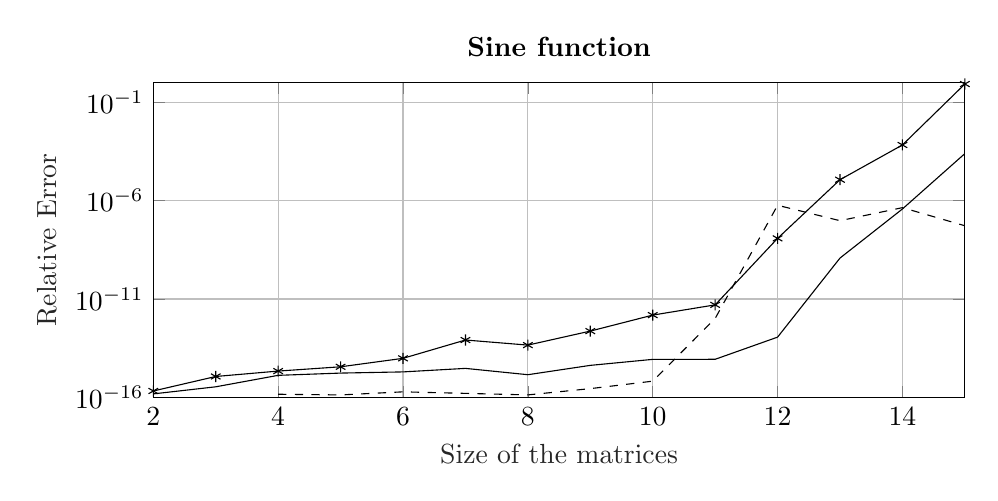
\begin{tikzpicture}

\begin{axis}[%
width=.85\linewidth,
height=4cm,
at={(0in,0in)},
scale only axis,
xmin=2,
xmax=15,
xlabel style={font=\color{white!15!black}},
xlabel={Size of the matrices},
ymode=log,
ymin=1e-16,
ymax=1,
yminorticks=true,
ylabel style={font=\color{white!15!black}},
ylabel={Relative Error},
axis background/.style={fill=white},
title style={font=\bfseries},
title={Sine function},
xmajorgrids,
ymajorgrids,
yminorgrids,
legend style={legend cell align=left, align=left, draw=white!15!black}
]
\addplot [color=black, dashed]
  table[row sep=crcr]{%
1	0\\
2	0\\
3	0\\
4	1.45725786217287e-16\\
5	1.34599448599507e-16\\
6	1.93288933939941e-16\\
7	0\\
8	1.34996517212839e-16\\
9	2.8139452012619e-16\\
10	6.73147337595159e-16\\
11	1.03032779116962e-12\\
12	5.78744177027967e-07\\
13	9.553747250617e-08\\
14	4.39017470636033e-07\\
15	5.28442449627079e-08\\
};
%\addlegendentry{diagonal}

\addplot [color=black, mark=asterisk, mark options={solid, black}]
  table[row sep=crcr]{%
1	0\\
2	2.13550872140361e-16\\
3	1.16425372303465e-15\\
4	2.19221444950359e-15\\
5	3.61672445574946e-15\\
6	9.72750676886519e-15\\
7	8.29608424074529e-14\\
8	4.56885037269095e-14\\
9	2.35417884883477e-13\\
10	1.52796832107972e-12\\
11	5.06284131371555e-12\\
12	1.20831615925066e-08\\
13	1.15240427666526e-05\\
14	0.000671713459124643\\
15	0.837016575460994\\
};
%\addlegendentry{symmetric}

\addplot [color=black]
  table[row sep=crcr]{%
1	0\\
2	1.51944372493216e-16\\
3	3.48056882596735e-16\\
4	1.33057104500803e-15\\
5	1.73250362957786e-15\\
6	1.99001209845091e-15\\
7	3.0020193056546e-15\\
8	1.43307608835298e-15\\
9	4.27119186288929e-15\\
10	8.62089393846284e-15\\
11	8.69296395513068e-15\\
12	1.16168249112529e-13\\
13	1.20836095810293e-09\\
14	3.76245413376949e-07\\
15	0.000244683076230114\\
};
%\addlegendentry{dense}

\end{axis}
\end{tikzpicture}%
        \caption{}
        \label{fig:comp_sine}
    \end{subfigure}\hspace{.055\linewidth}
    \begin{subfigure}[b]{0.3\textwidth}
        % This file was created by matlab2tikz.
%
%The latest updates can be retrieved from
%  http://www.mathworks.com/matlabcentral/fileexchange/22022-matlab2tikz-matlab2tikz
%where you can also make suggestions and rate matlab2tikz.
%
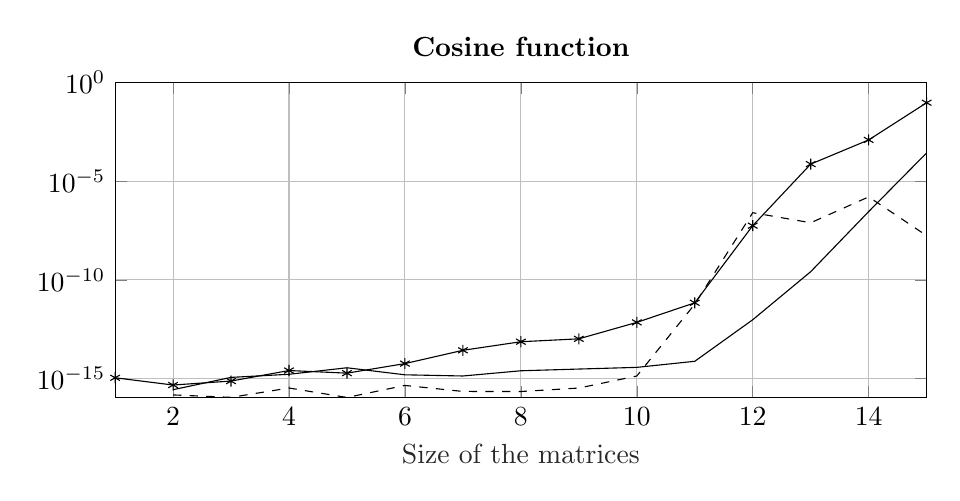
\begin{tikzpicture}

\begin{axis}[%
width=.85\linewidth,
height=4cm,
at={(0in,0in)},
scale only axis,
xmin=1,
xmax=15,
xlabel style={font=\color{white!15!black}},
xlabel={Size of the matrices},
ymode=log,
ymin=1.1104582787894e-16,
ymax=1,
yminorticks=true,
ylabel style={font=\color{white!15!black}},
%ylabel={Relative Error},
axis background/.style={fill=white},
title style={font=\bfseries},
title={Cosine function},
xmajorgrids,
ymajorgrids,
yminorgrids,
legend style={legend cell align=left, align=left, draw=white!15!black}
]
\addplot [color=black, dashed]
  table[row sep=crcr]{%
1	0\\
2	1.49254976159848e-16\\
3	1.12386960222902e-16\\
4	3.33629533162353e-16\\
5	1.1104582787894e-16\\
6	4.51664304824148e-16\\
7	2.24222591598726e-16\\
8	2.22284366724468e-16\\
9	3.3326394200314e-16\\
10	1.35535886136552e-15\\
11	5.90120769250069e-12\\
12	2.53895186073711e-07\\
13	7.86074239881932e-08\\
14	1.60599491859353e-06\\
15	1.74974849891932e-08\\
};
%\addlegendentry{diagonal}

\addplot [color=black, mark=asterisk, mark options={solid, black}]
  table[row sep=crcr]{%
1	1.10216884990089e-15\\
2	4.73392519955033e-16\\
3	7.52201284293378e-16\\
4	2.56983598583253e-15\\
5	1.8934958043445e-15\\
6	5.76079452953616e-15\\
7	2.71936809409104e-14\\
8	7.38660809880766e-14\\
9	1.03575975843225e-13\\
10	7.05810087502504e-13\\
11	6.91539504160167e-12\\
12	5.58866941125034e-08\\
13	7.35834262695204e-05\\
14	0.00123336328753215\\
15	0.0944453153509049\\
};
%\addlegendentry{symmetric}

\addplot [color=black]
  table[row sep=crcr]{%
1	0\\
2	2.74801956341246e-16\\
3	1.15411270860285e-15\\
4	1.65853388726515e-15\\
5	3.54103245149018e-15\\
6	1.5589802910102e-15\\
7	1.35811075119445e-15\\
8	2.49648348011263e-15\\
9	3.05245869225958e-15\\
10	3.71275847951212e-15\\
11	7.54587960659731e-15\\
12	9.59882062625648e-13\\
13	2.61418513595533e-10\\
14	2.89445409507326e-07\\
15	0.000271321657431055\\
};
%\addlegendentry{dense}

\end{axis}
\end{tikzpicture}%
        \caption{}
        \label{fig:comp_cosine}
    \end{subfigure}\hspace{.025\linewidth}
    \begin{subfigure}[b]{0.3\textwidth}
        % This file was created by matlab2tikz.
%
%The latest updates can be retrieved from
%  http://www.mathworks.com/matlabcentral/fileexchange/22022-matlab2tikz-matlab2tikz
%where you can also make suggestions and rate matlab2tikz.
%
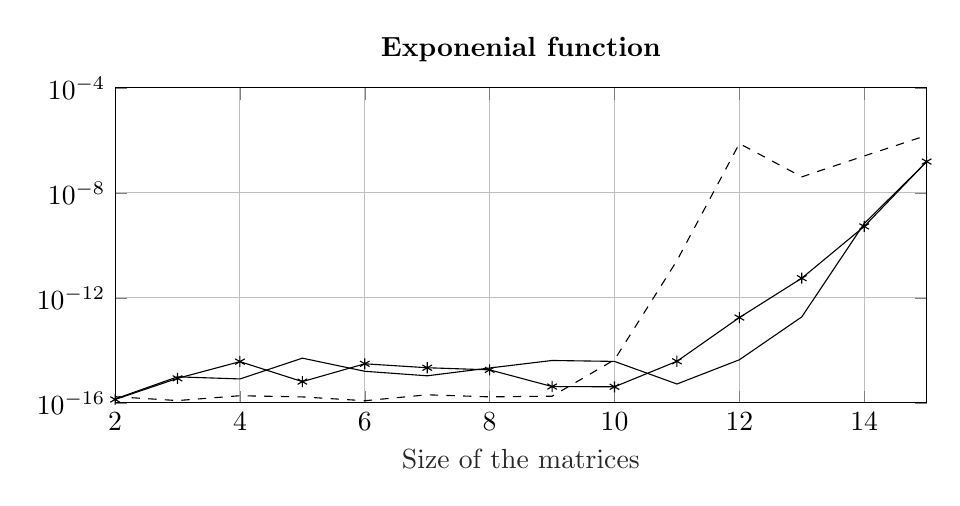
\begin{tikzpicture}

\begin{axis}[%
width=.85\linewidth,
height=4cm,
at={(0in,0in)},
scale only axis,
xmin=2,
xmax=15,
xlabel style={font=\color{white!15!black}},
xlabel={Size of the matrices},
ymode=log,
ymin=1e-16,
ymax=0.0001,
yminorticks=true,
ylabel style={font=\color{white!15!black}},
%ylabel={Relative Error},
axis background/.style={fill=white},
title style={font=\bfseries},
title={Exponenial function},
xmajorgrids,
ymajorgrids,
yminorgrids,
legend style={legend cell align=left, align=left, draw=white!15!black}
]
\addplot [color=black, dashed]
  table[row sep=crcr]{%
1	0\\
2	1.71624878976539e-16\\
3	1.22024250623032e-16\\
4	1.86764659618892e-16\\
5	1.68361863632822e-16\\
6	1.20424787755581e-16\\
7	2.02522198739353e-16\\
8	1.69083627914502e-16\\
9	1.78878188543304e-16\\
10	4.37883232600663e-15\\
11	2.62205407924652e-11\\
12	7.55548252824038e-07\\
13	4.08147804640456e-08\\
14	2.54902728221652e-07\\
15	1.54338995955608e-06\\
};
%\addlegendentry{diagonal}

\addplot [color=black, mark=asterisk, mark options={solid, black}]
  table[row sep=crcr]{%
1	0\\
2	1.34551194988101e-16\\
3	8.56940672084931e-16\\
4	3.71431920865263e-15\\
5	6.43853140792487e-16\\
6	3.07364008605186e-15\\
7	2.17447874006037e-15\\
8	1.80680598636716e-15\\
9	4.18315732440152e-16\\
10	4.08961300873358e-16\\
11	3.83448312676478e-15\\
12	1.77593347794744e-13\\
13	5.61443457608614e-12\\
14	5.25277002444549e-10\\
15	1.55722814732103e-07\\
};
%\addlegendentry{symmetric}

\addplot [color=black]
  table[row sep=crcr]{%
1	0\\
2	1.40422527187022e-16\\
3	9.78212455490046e-16\\
4	8.14581110397033e-16\\
5	5.04209119228841e-15\\
6	1.59210015961528e-15\\
7	1.07228002023245e-15\\
8	2.12873989764519e-15\\
9	4.11404419473943e-15\\
10	3.79263905604626e-15\\
11	5.22236059957374e-16\\
12	4.37354475237039e-15\\
13	1.88271014260457e-13\\
14	6.79585192457534e-10\\
15	1.52106181005324e-07\\
};
%\addlegendentry{dense}

\end{axis}
\end{tikzpicture}%
        \caption{}
        \label{fig:comp_exp}
    \end{subfigure}
    \caption{Measure of performance of the algorithm to compute $f(\mathbf{A})$ according to definition \ref{def:Hermite}. We assume that \cite{davies2003schur} (Schur Parlett) algorithm is correct, and we measure the relative error. We compare the performance of our algorithm on several types of matrices : diagonal (- -), symmetric (-*) and dense (--). Matrix coefficients are randomly filled such that for all non-zero entry: $a_{ij}\sim\mathcal{U}(0,1)$, this ensures $\mathbf{A}$ is full rank. We test it on three different functions : Sine (a), Cosine (b) and Exponenial (c). We note that starting from a certain matrix size, the algorithm lose considerably in performance.}
    \label{fig:comp}
\end{figure}

Figure \ref{fig:comp} illustrates the result of the measurement of performance of the algorithm. The relative error between \cite{davies2003schur} and our results is computed:
\begin{equation*}
    \text{relative error} = \frac{\|f(\mathbf{A})-\texttt{funm}(\mathbf{A},f)\|_2}{\|\texttt{funm}(\mathbf{A},f\|_2}
\end{equation*}
We note that for small matrices ($n\leq 10$), the hermite interpolation approach is precise and has residual error inferior to $10^{-11}$, which is somewhat close to numerical precision (around $10^{-16}$ as we work with double precision). However, starting from a certain matrix size, the algorithm loses considerably in performance: both in precision and in computation time. Interestingly, this behavior is independant to the matrix structure : diagonal, symmetric or dense. It also seem to be independant to the function we are evaluating (though we has slightly lower relative error for the exponential function as depicted in figure \ref{fig:comp_exp}).

We conclude that this algorithm, while being elegant, is quickly inefficient, and lead to both numerical and computational issues, even at small matrix sizes.

\subsection{Matrix-vector product}
\subsubsection{Implementation}
In this section, we will implement the matrix-vector product $f(\mathbf{A})\mathbf{b}$, as described in section \ref{sec:fabintro}. We will use the Arnoldi method to achieve this. The implementation is done in \texttt{Matlab 2023a}. As the theory has been well described in section \ref{sec:fabintro}, the implementation is straight-forward :
\begin{algorithm2e}
    \SetAlgoLined
    \KwData{$\mathbf{A} \in \mathbb{C}^{n \times n}$, $\mathbf{b} \in \mathbb{C}^n$, $f$ a function and $k\in\mathbb{N}$ the dimension of the Krylov subspace}
    \KwResult{$f(\mathbf{A})\mathbf{b}$}
    \caption{Matrix-Vector Product}
    $\mathbf{v}_1 \gets \mathbf{b}/\|\mathbf{b}\|_2$\;
    $[\mathbf{V},\mathbf{H}] \gets$ \texttt{arnoldi}($\mathbf{A},\mathbf{v}_1,k$)\;
    $e_1 \gets$ first column of the identity matrix\;
    $f \gets \|b\|_2\mathbf{V}f(\mathbf{H})\mathbf{e}_1$\;
\end{algorithm2e}

Where \texttt{arnoldi()} is the Arnoldi iteration described in algorithm \ref{alg:arnoldi}. This routine is provided in the supplementary materials.

\subsubsection{Results}
To evaluate the performance of this Matrix-vector product routine, we will test it versus the naive way of doing it in \texttt{Matlab}, meaning computing $f(\mathbf{A})$ explicitely, then multiplying it by $\mathbf{b}$. In our first experiment (figure \ref{fig:comp_fab}), where $\mathbf{A}$ is a large sparse matrix. More specifically it is a graded L-shape pattern from \cite{george1978automatic}. The vector $\mathbf{b}$ is filled with uniformly distributed random coefficients such that $b_i\sim\mathcal{U}(0,1)$. The figure \ref{fig:comp_fab_assignement} shows that for such a setup, the proposed algorithm reaches a relative error equals to numerical precision few iterations afters 20. This means 
\begin{equation*}
    \frac{\|\|\mathbf{b}\|_2\mathbf{V}_k f(\mathbf{H}_k)\mathbf{e}_1 - f(\mathbf{A})\mathbf{b}\|_2}{\|f(\mathbf{A})\mathbf{b}\|_2} = \epsilon
\end{equation*}
for $k > 20$, and where $\epsilon$ is the machine precision. Note that this result is very specific to the problem depicted in figure \ref{fig:comp_fab}, and the threshold for $k$ will differ in function of the considered problem. Another interpretation is that computing $f(\mathbf{A})\mathbf{b}$ on the smaller Krylov subspace $\mathcal{K}_k(\mathbf{A},\mathbf{b})$ gives extremely good results, even when $k << n$. 
\begin{figure}
    \begin{subfigure}[b]{.45\linewidth}
        % This file was created by matlab2tikz.
%
%The latest updates can be retrieved from
%  http://www.mathworks.com/matlabcentral/fileexchange/22022-matlab2tikz-matlab2tikz
%where you can also make suggestions and rate matlab2tikz.
%
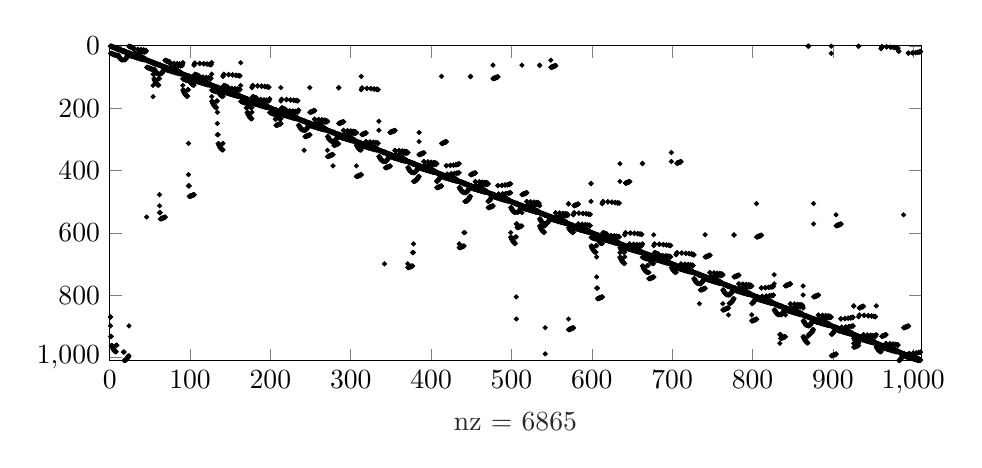
\begin{tikzpicture}

\begin{axis}[%
width=.85\linewidth,
height=4cm,
at={(0in,0in)},
scale only axis,
xmin=0,
xmax=1010,
xlabel style={font=\color{white!15!black}},
xlabel={nz = 6865},
y dir=reverse,
ymin=0,
ymax=1010,
axis background/.style={fill=white},
legend style={legend cell align=left, align=left, draw=white!15!black}
]
\addplot [color=black, draw=none, mark size=0.7pt, mark=*, mark options={solid, black}, forget plot]
  table[row sep=crcr]{%
1	1\\
1	2\\
1	24\\
1	869\\
1	870\\
1	898\\
1	932\\
2	1\\
2	2\\
2	3\\
2	24\\
2	25\\
2	932\\
2	961\\
3	2\\
3	3\\
3	4\\
3	25\\
3	26\\
3	961\\
3	967\\
4	3\\
4	4\\
4	5\\
4	26\\
4	27\\
4	967\\
4	972\\
5	4\\
5	5\\
5	6\\
5	27\\
5	28\\
5	972\\
5	976\\
6	5\\
6	6\\
6	7\\
6	28\\
6	29\\
6	976\\
6	979\\
7	6\\
7	7\\
7	8\\
7	29\\
7	30\\
7	979\\
7	981\\
8	7\\
8	8\\
8	9\\
8	10\\
8	30\\
8	960\\
8	981\\
9	8\\
9	9\\
9	10\\
9	960\\
10	8\\
10	9\\
10	10\\
10	11\\
10	30\\
11	10\\
11	11\\
11	12\\
11	30\\
11	35\\
12	11\\
12	12\\
12	13\\
12	35\\
12	39\\
13	12\\
13	13\\
13	14\\
13	39\\
13	42\\
14	13\\
14	14\\
14	15\\
14	42\\
14	44\\
15	14\\
15	15\\
15	16\\
15	44\\
15	45\\
16	15\\
16	16\\
16	17\\
16	18\\
16	45\\
17	16\\
17	17\\
17	18\\
17	982\\
18	16\\
18	17\\
18	18\\
18	19\\
18	45\\
18	982\\
18	1009\\
19	18\\
19	19\\
19	20\\
19	43\\
19	45\\
19	1008\\
19	1009\\
20	19\\
20	20\\
20	21\\
20	40\\
20	43\\
20	1006\\
20	1008\\
21	20\\
21	21\\
21	22\\
21	36\\
21	40\\
21	1003\\
21	1006\\
22	21\\
22	22\\
22	23\\
22	31\\
22	36\\
22	999\\
22	1003\\
23	22\\
23	23\\
23	24\\
23	25\\
23	31\\
23	994\\
23	999\\
24	1\\
24	2\\
24	23\\
24	24\\
24	25\\
24	898\\
24	994\\
25	2\\
25	3\\
25	23\\
25	24\\
25	25\\
25	26\\
25	31\\
26	3\\
26	4\\
26	25\\
26	26\\
26	27\\
26	31\\
26	32\\
27	4\\
27	5\\
27	26\\
27	27\\
27	28\\
27	32\\
27	33\\
28	5\\
28	6\\
28	27\\
28	28\\
28	29\\
28	33\\
28	34\\
29	6\\
29	7\\
29	28\\
29	29\\
29	30\\
29	34\\
29	35\\
30	7\\
30	8\\
30	10\\
30	11\\
30	29\\
30	30\\
30	35\\
31	22\\
31	23\\
31	25\\
31	26\\
31	31\\
31	32\\
31	36\\
32	26\\
32	27\\
32	31\\
32	32\\
32	33\\
32	36\\
32	37\\
33	27\\
33	28\\
33	32\\
33	33\\
33	34\\
33	37\\
33	38\\
34	28\\
34	29\\
34	33\\
34	34\\
34	35\\
34	38\\
34	39\\
35	11\\
35	12\\
35	29\\
35	30\\
35	34\\
35	35\\
35	39\\
36	21\\
36	22\\
36	31\\
36	32\\
36	36\\
36	37\\
36	40\\
37	32\\
37	33\\
37	36\\
37	37\\
37	38\\
37	40\\
37	41\\
38	33\\
38	34\\
38	37\\
38	38\\
38	39\\
38	41\\
38	42\\
39	12\\
39	13\\
39	34\\
39	35\\
39	38\\
39	39\\
39	42\\
40	20\\
40	21\\
40	36\\
40	37\\
40	40\\
40	41\\
40	43\\
41	37\\
41	38\\
41	40\\
41	41\\
41	42\\
41	43\\
41	44\\
42	13\\
42	14\\
42	38\\
42	39\\
42	41\\
42	42\\
42	44\\
43	19\\
43	20\\
43	40\\
43	41\\
43	43\\
43	44\\
43	45\\
44	14\\
44	15\\
44	41\\
44	42\\
44	43\\
44	44\\
44	45\\
45	15\\
45	16\\
45	18\\
45	19\\
45	43\\
45	44\\
45	45\\
46	46\\
46	47\\
46	69\\
46	549\\
47	46\\
47	47\\
47	48\\
47	69\\
47	70\\
48	47\\
48	48\\
48	49\\
48	70\\
48	71\\
49	48\\
49	49\\
49	50\\
49	71\\
49	72\\
50	49\\
50	50\\
50	51\\
50	72\\
50	73\\
51	50\\
51	51\\
51	52\\
51	73\\
51	74\\
52	51\\
52	52\\
52	53\\
52	74\\
52	75\\
53	52\\
53	53\\
53	54\\
53	55\\
53	75\\
54	53\\
54	54\\
54	55\\
54	91\\
54	127\\
54	163\\
55	53\\
55	54\\
55	55\\
55	56\\
55	75\\
55	91\\
55	106\\
56	55\\
56	56\\
56	57\\
56	75\\
56	80\\
56	106\\
56	112\\
57	56\\
57	57\\
57	58\\
57	80\\
57	84\\
57	112\\
57	117\\
58	57\\
58	58\\
58	59\\
58	84\\
58	87\\
58	117\\
58	121\\
59	58\\
59	59\\
59	60\\
59	87\\
59	89\\
59	121\\
59	124\\
60	59\\
60	60\\
60	61\\
60	89\\
60	90\\
60	124\\
60	126\\
61	60\\
61	61\\
61	62\\
61	63\\
61	90\\
61	105\\
61	126\\
62	61\\
62	62\\
62	63\\
62	105\\
62	477\\
62	513\\
62	535\\
63	61\\
63	62\\
63	63\\
63	64\\
63	90\\
63	535\\
63	555\\
64	63\\
64	64\\
64	65\\
64	88\\
64	90\\
64	554\\
64	555\\
65	64\\
65	65\\
65	66\\
65	85\\
65	88\\
65	553\\
65	554\\
66	65\\
66	66\\
66	67\\
66	81\\
66	85\\
66	552\\
66	553\\
67	66\\
67	67\\
67	68\\
67	76\\
67	81\\
67	551\\
67	552\\
68	67\\
68	68\\
68	69\\
68	70\\
68	76\\
68	550\\
68	551\\
69	46\\
69	47\\
69	68\\
69	69\\
69	70\\
69	549\\
69	550\\
70	47\\
70	48\\
70	68\\
70	69\\
70	70\\
70	71\\
70	76\\
71	48\\
71	49\\
71	70\\
71	71\\
71	72\\
71	76\\
71	77\\
72	49\\
72	50\\
72	71\\
72	72\\
72	73\\
72	77\\
72	78\\
73	50\\
73	51\\
73	72\\
73	73\\
73	74\\
73	78\\
73	79\\
74	51\\
74	52\\
74	73\\
74	74\\
74	75\\
74	79\\
74	80\\
75	52\\
75	53\\
75	55\\
75	56\\
75	74\\
75	75\\
75	80\\
76	67\\
76	68\\
76	70\\
76	71\\
76	76\\
76	77\\
76	81\\
77	71\\
77	72\\
77	76\\
77	77\\
77	78\\
77	81\\
77	82\\
78	72\\
78	73\\
78	77\\
78	78\\
78	79\\
78	82\\
78	83\\
79	73\\
79	74\\
79	78\\
79	79\\
79	80\\
79	83\\
79	84\\
80	56\\
80	57\\
80	74\\
80	75\\
80	79\\
80	80\\
80	84\\
81	66\\
81	67\\
81	76\\
81	77\\
81	81\\
81	82\\
81	85\\
82	77\\
82	78\\
82	81\\
82	82\\
82	83\\
82	85\\
82	86\\
83	78\\
83	79\\
83	82\\
83	83\\
83	84\\
83	86\\
83	87\\
84	57\\
84	58\\
84	79\\
84	80\\
84	83\\
84	84\\
84	87\\
85	65\\
85	66\\
85	81\\
85	82\\
85	85\\
85	86\\
85	88\\
86	82\\
86	83\\
86	85\\
86	86\\
86	87\\
86	88\\
86	89\\
87	58\\
87	59\\
87	83\\
87	84\\
87	86\\
87	87\\
87	89\\
88	64\\
88	65\\
88	85\\
88	86\\
88	88\\
88	89\\
88	90\\
89	59\\
89	60\\
89	86\\
89	87\\
89	88\\
89	89\\
89	90\\
90	60\\
90	61\\
90	63\\
90	64\\
90	88\\
90	89\\
90	90\\
91	54\\
91	55\\
91	91\\
91	92\\
91	106\\
91	127\\
91	142\\
92	91\\
92	92\\
92	93\\
92	106\\
92	107\\
92	142\\
92	148\\
93	92\\
93	93\\
93	94\\
93	107\\
93	108\\
93	148\\
93	153\\
94	93\\
94	94\\
94	95\\
94	108\\
94	109\\
94	153\\
94	157\\
95	94\\
95	95\\
95	96\\
95	109\\
95	110\\
95	157\\
95	160\\
96	95\\
96	96\\
96	97\\
96	110\\
96	111\\
96	160\\
96	162\\
97	96\\
97	97\\
97	98\\
97	99\\
97	111\\
97	141\\
97	162\\
98	97\\
98	98\\
98	99\\
98	141\\
98	313\\
98	413\\
98	449\\
99	97\\
99	98\\
99	99\\
99	100\\
99	111\\
99	449\\
99	483\\
100	99\\
100	100\\
100	101\\
100	111\\
100	116\\
100	482\\
100	483\\
101	100\\
101	101\\
101	102\\
101	116\\
101	120\\
101	481\\
101	482\\
102	101\\
102	102\\
102	103\\
102	120\\
102	123\\
102	480\\
102	481\\
103	102\\
103	103\\
103	104\\
103	123\\
103	125\\
103	479\\
103	480\\
104	103\\
104	104\\
104	105\\
104	125\\
104	126\\
104	478\\
104	479\\
105	61\\
105	62\\
105	104\\
105	105\\
105	126\\
105	477\\
105	478\\
106	55\\
106	56\\
106	91\\
106	92\\
106	106\\
106	107\\
106	112\\
107	92\\
107	93\\
107	106\\
107	107\\
107	108\\
107	112\\
107	113\\
108	93\\
108	94\\
108	107\\
108	108\\
108	109\\
108	113\\
108	114\\
109	94\\
109	95\\
109	108\\
109	109\\
109	110\\
109	114\\
109	115\\
110	95\\
110	96\\
110	109\\
110	110\\
110	111\\
110	115\\
110	116\\
111	96\\
111	97\\
111	99\\
111	100\\
111	110\\
111	111\\
111	116\\
112	56\\
112	57\\
112	106\\
112	107\\
112	112\\
112	113\\
112	117\\
113	107\\
113	108\\
113	112\\
113	113\\
113	114\\
113	117\\
113	118\\
114	108\\
114	109\\
114	113\\
114	114\\
114	115\\
114	118\\
114	119\\
115	109\\
115	110\\
115	114\\
115	115\\
115	116\\
115	119\\
115	120\\
116	100\\
116	101\\
116	110\\
116	111\\
116	115\\
116	116\\
116	120\\
117	57\\
117	58\\
117	112\\
117	113\\
117	117\\
117	118\\
117	121\\
118	113\\
118	114\\
118	117\\
118	118\\
118	119\\
118	121\\
118	122\\
119	114\\
119	115\\
119	118\\
119	119\\
119	120\\
119	122\\
119	123\\
120	101\\
120	102\\
120	115\\
120	116\\
120	119\\
120	120\\
120	123\\
121	58\\
121	59\\
121	117\\
121	118\\
121	121\\
121	122\\
121	124\\
122	118\\
122	119\\
122	121\\
122	122\\
122	123\\
122	124\\
122	125\\
123	102\\
123	103\\
123	119\\
123	120\\
123	122\\
123	123\\
123	125\\
124	59\\
124	60\\
124	121\\
124	122\\
124	124\\
124	125\\
124	126\\
125	103\\
125	104\\
125	122\\
125	123\\
125	124\\
125	125\\
125	126\\
126	60\\
126	61\\
126	104\\
126	105\\
126	124\\
126	125\\
126	126\\
127	54\\
127	91\\
127	127\\
127	128\\
127	142\\
127	163\\
127	178\\
128	127\\
128	128\\
128	129\\
128	142\\
128	143\\
128	178\\
128	184\\
129	128\\
129	129\\
129	130\\
129	143\\
129	144\\
129	184\\
129	189\\
130	129\\
130	130\\
130	131\\
130	144\\
130	145\\
130	189\\
130	193\\
131	130\\
131	131\\
131	132\\
131	145\\
131	146\\
131	193\\
131	196\\
132	131\\
132	132\\
132	133\\
132	146\\
132	147\\
132	196\\
132	198\\
133	132\\
133	133\\
133	134\\
133	135\\
133	147\\
133	177\\
133	198\\
134	133\\
134	134\\
134	135\\
134	177\\
134	213\\
134	249\\
134	285\\
135	133\\
135	134\\
135	135\\
135	136\\
135	147\\
135	285\\
135	314\\
136	135\\
136	136\\
136	137\\
136	147\\
136	152\\
136	314\\
136	320\\
137	136\\
137	137\\
137	138\\
137	152\\
137	156\\
137	320\\
137	325\\
138	137\\
138	138\\
138	139\\
138	156\\
138	159\\
138	325\\
138	329\\
139	138\\
139	139\\
139	140\\
139	159\\
139	161\\
139	329\\
139	332\\
140	139\\
140	140\\
140	141\\
140	161\\
140	162\\
140	332\\
140	334\\
141	97\\
141	98\\
141	140\\
141	141\\
141	162\\
141	313\\
141	334\\
142	91\\
142	92\\
142	127\\
142	128\\
142	142\\
142	143\\
142	148\\
143	128\\
143	129\\
143	142\\
143	143\\
143	144\\
143	148\\
143	149\\
144	129\\
144	130\\
144	143\\
144	144\\
144	145\\
144	149\\
144	150\\
145	130\\
145	131\\
145	144\\
145	145\\
145	146\\
145	150\\
145	151\\
146	131\\
146	132\\
146	145\\
146	146\\
146	147\\
146	151\\
146	152\\
147	132\\
147	133\\
147	135\\
147	136\\
147	146\\
147	147\\
147	152\\
148	92\\
148	93\\
148	142\\
148	143\\
148	148\\
148	149\\
148	153\\
149	143\\
149	144\\
149	148\\
149	149\\
149	150\\
149	153\\
149	154\\
150	144\\
150	145\\
150	149\\
150	150\\
150	151\\
150	154\\
150	155\\
151	145\\
151	146\\
151	150\\
151	151\\
151	152\\
151	155\\
151	156\\
152	136\\
152	137\\
152	146\\
152	147\\
152	151\\
152	152\\
152	156\\
153	93\\
153	94\\
153	148\\
153	149\\
153	153\\
153	154\\
153	157\\
154	149\\
154	150\\
154	153\\
154	154\\
154	155\\
154	157\\
154	158\\
155	150\\
155	151\\
155	154\\
155	155\\
155	156\\
155	158\\
155	159\\
156	137\\
156	138\\
156	151\\
156	152\\
156	155\\
156	156\\
156	159\\
157	94\\
157	95\\
157	153\\
157	154\\
157	157\\
157	158\\
157	160\\
158	154\\
158	155\\
158	157\\
158	158\\
158	159\\
158	160\\
158	161\\
159	138\\
159	139\\
159	155\\
159	156\\
159	158\\
159	159\\
159	161\\
160	95\\
160	96\\
160	157\\
160	158\\
160	160\\
160	161\\
160	162\\
161	139\\
161	140\\
161	158\\
161	159\\
161	160\\
161	161\\
161	162\\
162	96\\
162	97\\
162	140\\
162	141\\
162	160\\
162	161\\
162	162\\
163	54\\
163	127\\
163	163\\
163	164\\
163	178\\
164	163\\
164	164\\
164	165\\
164	178\\
164	179\\
165	164\\
165	165\\
165	166\\
165	179\\
165	180\\
166	165\\
166	166\\
166	167\\
166	180\\
166	181\\
167	166\\
167	167\\
167	168\\
167	181\\
167	182\\
168	167\\
168	168\\
168	169\\
168	182\\
168	183\\
169	168\\
169	169\\
169	170\\
169	171\\
169	183\\
170	169\\
170	170\\
170	171\\
170	199\\
171	169\\
171	170\\
171	171\\
171	172\\
171	183\\
171	199\\
171	214\\
172	171\\
172	172\\
172	173\\
172	183\\
172	188\\
172	214\\
172	220\\
173	172\\
173	173\\
173	174\\
173	188\\
173	192\\
173	220\\
173	225\\
174	173\\
174	174\\
174	175\\
174	192\\
174	195\\
174	225\\
174	229\\
175	174\\
175	175\\
175	176\\
175	195\\
175	197\\
175	229\\
175	232\\
176	175\\
176	176\\
176	177\\
176	197\\
176	198\\
176	232\\
176	234\\
177	133\\
177	134\\
177	176\\
177	177\\
177	198\\
177	213\\
177	234\\
178	127\\
178	128\\
178	163\\
178	164\\
178	178\\
178	179\\
178	184\\
179	164\\
179	165\\
179	178\\
179	179\\
179	180\\
179	184\\
179	185\\
180	165\\
180	166\\
180	179\\
180	180\\
180	181\\
180	185\\
180	186\\
181	166\\
181	167\\
181	180\\
181	181\\
181	182\\
181	186\\
181	187\\
182	167\\
182	168\\
182	181\\
182	182\\
182	183\\
182	187\\
182	188\\
183	168\\
183	169\\
183	171\\
183	172\\
183	182\\
183	183\\
183	188\\
184	128\\
184	129\\
184	178\\
184	179\\
184	184\\
184	185\\
184	189\\
185	179\\
185	180\\
185	184\\
185	185\\
185	186\\
185	189\\
185	190\\
186	180\\
186	181\\
186	185\\
186	186\\
186	187\\
186	190\\
186	191\\
187	181\\
187	182\\
187	186\\
187	187\\
187	188\\
187	191\\
187	192\\
188	172\\
188	173\\
188	182\\
188	183\\
188	187\\
188	188\\
188	192\\
189	129\\
189	130\\
189	184\\
189	185\\
189	189\\
189	190\\
189	193\\
190	185\\
190	186\\
190	189\\
190	190\\
190	191\\
190	193\\
190	194\\
191	186\\
191	187\\
191	190\\
191	191\\
191	192\\
191	194\\
191	195\\
192	173\\
192	174\\
192	187\\
192	188\\
192	191\\
192	192\\
192	195\\
193	130\\
193	131\\
193	189\\
193	190\\
193	193\\
193	194\\
193	196\\
194	190\\
194	191\\
194	193\\
194	194\\
194	195\\
194	196\\
194	197\\
195	174\\
195	175\\
195	191\\
195	192\\
195	194\\
195	195\\
195	197\\
196	131\\
196	132\\
196	193\\
196	194\\
196	196\\
196	197\\
196	198\\
197	175\\
197	176\\
197	194\\
197	195\\
197	196\\
197	197\\
197	198\\
198	132\\
198	133\\
198	176\\
198	177\\
198	196\\
198	197\\
198	198\\
199	170\\
199	171\\
199	199\\
199	200\\
199	214\\
200	199\\
200	200\\
200	201\\
200	214\\
200	215\\
201	200\\
201	201\\
201	202\\
201	215\\
201	216\\
202	201\\
202	202\\
202	203\\
202	216\\
202	217\\
203	202\\
203	203\\
203	204\\
203	217\\
203	218\\
204	203\\
204	204\\
204	205\\
204	218\\
204	219\\
205	204\\
205	205\\
205	206\\
205	207\\
205	219\\
206	205\\
206	206\\
206	207\\
206	235\\
207	205\\
207	206\\
207	207\\
207	208\\
207	219\\
207	235\\
207	255\\
208	207\\
208	208\\
208	209\\
208	219\\
208	224\\
208	254\\
208	255\\
209	208\\
209	209\\
209	210\\
209	224\\
209	228\\
209	253\\
209	254\\
210	209\\
210	210\\
210	211\\
210	228\\
210	231\\
210	252\\
210	253\\
211	210\\
211	211\\
211	212\\
211	231\\
211	233\\
211	251\\
211	252\\
212	211\\
212	212\\
212	213\\
212	233\\
212	234\\
212	250\\
212	251\\
213	134\\
213	177\\
213	212\\
213	213\\
213	234\\
213	249\\
213	250\\
214	171\\
214	172\\
214	199\\
214	200\\
214	214\\
214	215\\
214	220\\
215	200\\
215	201\\
215	214\\
215	215\\
215	216\\
215	220\\
215	221\\
216	201\\
216	202\\
216	215\\
216	216\\
216	217\\
216	221\\
216	222\\
217	202\\
217	203\\
217	216\\
217	217\\
217	218\\
217	222\\
217	223\\
218	203\\
218	204\\
218	217\\
218	218\\
218	219\\
218	223\\
218	224\\
219	204\\
219	205\\
219	207\\
219	208\\
219	218\\
219	219\\
219	224\\
220	172\\
220	173\\
220	214\\
220	215\\
220	220\\
220	221\\
220	225\\
221	215\\
221	216\\
221	220\\
221	221\\
221	222\\
221	225\\
221	226\\
222	216\\
222	217\\
222	221\\
222	222\\
222	223\\
222	226\\
222	227\\
223	217\\
223	218\\
223	222\\
223	223\\
223	224\\
223	227\\
223	228\\
224	208\\
224	209\\
224	218\\
224	219\\
224	223\\
224	224\\
224	228\\
225	173\\
225	174\\
225	220\\
225	221\\
225	225\\
225	226\\
225	229\\
226	221\\
226	222\\
226	225\\
226	226\\
226	227\\
226	229\\
226	230\\
227	222\\
227	223\\
227	226\\
227	227\\
227	228\\
227	230\\
227	231\\
228	209\\
228	210\\
228	223\\
228	224\\
228	227\\
228	228\\
228	231\\
229	174\\
229	175\\
229	225\\
229	226\\
229	229\\
229	230\\
229	232\\
230	226\\
230	227\\
230	229\\
230	230\\
230	231\\
230	232\\
230	233\\
231	210\\
231	211\\
231	227\\
231	228\\
231	230\\
231	231\\
231	233\\
232	175\\
232	176\\
232	229\\
232	230\\
232	232\\
232	233\\
232	234\\
233	211\\
233	212\\
233	230\\
233	231\\
233	232\\
233	233\\
233	234\\
234	176\\
234	177\\
234	212\\
234	213\\
234	232\\
234	233\\
234	234\\
235	206\\
235	207\\
235	235\\
235	236\\
235	255\\
236	235\\
236	236\\
236	237\\
236	255\\
236	260\\
237	236\\
237	237\\
237	238\\
237	260\\
237	264\\
238	237\\
238	238\\
238	239\\
238	264\\
238	267\\
239	238\\
239	239\\
239	240\\
239	267\\
239	269\\
240	239\\
240	240\\
240	241\\
240	269\\
240	270\\
241	240\\
241	241\\
241	242\\
241	243\\
241	270\\
242	241\\
242	242\\
242	243\\
242	271\\
242	335\\
243	241\\
243	242\\
243	243\\
243	244\\
243	270\\
243	271\\
243	291\\
244	243\\
244	244\\
244	245\\
244	268\\
244	270\\
244	290\\
244	291\\
245	244\\
245	245\\
245	246\\
245	265\\
245	268\\
245	289\\
245	290\\
246	245\\
246	246\\
246	247\\
246	261\\
246	265\\
246	288\\
246	289\\
247	246\\
247	247\\
247	248\\
247	256\\
247	261\\
247	287\\
247	288\\
248	247\\
248	248\\
248	249\\
248	250\\
248	256\\
248	286\\
248	287\\
249	134\\
249	213\\
249	248\\
249	249\\
249	250\\
249	285\\
249	286\\
250	212\\
250	213\\
250	248\\
250	249\\
250	250\\
250	251\\
250	256\\
251	211\\
251	212\\
251	250\\
251	251\\
251	252\\
251	256\\
251	257\\
252	210\\
252	211\\
252	251\\
252	252\\
252	253\\
252	257\\
252	258\\
253	209\\
253	210\\
253	252\\
253	253\\
253	254\\
253	258\\
253	259\\
254	208\\
254	209\\
254	253\\
254	254\\
254	255\\
254	259\\
254	260\\
255	207\\
255	208\\
255	235\\
255	236\\
255	254\\
255	255\\
255	260\\
256	247\\
256	248\\
256	250\\
256	251\\
256	256\\
256	257\\
256	261\\
257	251\\
257	252\\
257	256\\
257	257\\
257	258\\
257	261\\
257	262\\
258	252\\
258	253\\
258	257\\
258	258\\
258	259\\
258	262\\
258	263\\
259	253\\
259	254\\
259	258\\
259	259\\
259	260\\
259	263\\
259	264\\
260	236\\
260	237\\
260	254\\
260	255\\
260	259\\
260	260\\
260	264\\
261	246\\
261	247\\
261	256\\
261	257\\
261	261\\
261	262\\
261	265\\
262	257\\
262	258\\
262	261\\
262	262\\
262	263\\
262	265\\
262	266\\
263	258\\
263	259\\
263	262\\
263	263\\
263	264\\
263	266\\
263	267\\
264	237\\
264	238\\
264	259\\
264	260\\
264	263\\
264	264\\
264	267\\
265	245\\
265	246\\
265	261\\
265	262\\
265	265\\
265	266\\
265	268\\
266	262\\
266	263\\
266	265\\
266	266\\
266	267\\
266	268\\
266	269\\
267	238\\
267	239\\
267	263\\
267	264\\
267	266\\
267	267\\
267	269\\
268	244\\
268	245\\
268	265\\
268	266\\
268	268\\
268	269\\
268	270\\
269	239\\
269	240\\
269	266\\
269	267\\
269	268\\
269	269\\
269	270\\
270	240\\
270	241\\
270	243\\
270	244\\
270	268\\
270	269\\
270	270\\
271	242\\
271	243\\
271	271\\
271	272\\
271	291\\
271	335\\
271	355\\
272	271\\
272	272\\
272	273\\
272	291\\
272	296\\
272	354\\
272	355\\
273	272\\
273	273\\
273	274\\
273	296\\
273	300\\
273	353\\
273	354\\
274	273\\
274	274\\
274	275\\
274	300\\
274	303\\
274	352\\
274	353\\
275	274\\
275	275\\
275	276\\
275	303\\
275	305\\
275	351\\
275	352\\
276	275\\
276	276\\
276	277\\
276	305\\
276	306\\
276	350\\
276	351\\
277	276\\
277	277\\
277	278\\
277	279\\
277	306\\
277	349\\
277	350\\
278	277\\
278	278\\
278	279\\
278	307\\
278	349\\
278	385\\
279	277\\
279	278\\
279	279\\
279	280\\
279	306\\
279	307\\
279	319\\
280	279\\
280	280\\
280	281\\
280	304\\
280	306\\
280	318\\
280	319\\
281	280\\
281	281\\
281	282\\
281	301\\
281	304\\
281	317\\
281	318\\
282	281\\
282	282\\
282	283\\
282	297\\
282	301\\
282	316\\
282	317\\
283	282\\
283	283\\
283	284\\
283	292\\
283	297\\
283	315\\
283	316\\
284	283\\
284	284\\
284	285\\
284	286\\
284	292\\
284	314\\
284	315\\
285	134\\
285	135\\
285	249\\
285	284\\
285	285\\
285	286\\
285	314\\
286	248\\
286	249\\
286	284\\
286	285\\
286	286\\
286	287\\
286	292\\
287	247\\
287	248\\
287	286\\
287	287\\
287	288\\
287	292\\
287	293\\
288	246\\
288	247\\
288	287\\
288	288\\
288	289\\
288	293\\
288	294\\
289	245\\
289	246\\
289	288\\
289	289\\
289	290\\
289	294\\
289	295\\
290	244\\
290	245\\
290	289\\
290	290\\
290	291\\
290	295\\
290	296\\
291	243\\
291	244\\
291	271\\
291	272\\
291	290\\
291	291\\
291	296\\
292	283\\
292	284\\
292	286\\
292	287\\
292	292\\
292	293\\
292	297\\
293	287\\
293	288\\
293	292\\
293	293\\
293	294\\
293	297\\
293	298\\
294	288\\
294	289\\
294	293\\
294	294\\
294	295\\
294	298\\
294	299\\
295	289\\
295	290\\
295	294\\
295	295\\
295	296\\
295	299\\
295	300\\
296	272\\
296	273\\
296	290\\
296	291\\
296	295\\
296	296\\
296	300\\
297	282\\
297	283\\
297	292\\
297	293\\
297	297\\
297	298\\
297	301\\
298	293\\
298	294\\
298	297\\
298	298\\
298	299\\
298	301\\
298	302\\
299	294\\
299	295\\
299	298\\
299	299\\
299	300\\
299	302\\
299	303\\
300	273\\
300	274\\
300	295\\
300	296\\
300	299\\
300	300\\
300	303\\
301	281\\
301	282\\
301	297\\
301	298\\
301	301\\
301	302\\
301	304\\
302	298\\
302	299\\
302	301\\
302	302\\
302	303\\
302	304\\
302	305\\
303	274\\
303	275\\
303	299\\
303	300\\
303	302\\
303	303\\
303	305\\
304	280\\
304	281\\
304	301\\
304	302\\
304	304\\
304	305\\
304	306\\
305	275\\
305	276\\
305	302\\
305	303\\
305	304\\
305	305\\
305	306\\
306	276\\
306	277\\
306	279\\
306	280\\
306	304\\
306	305\\
306	306\\
307	278\\
307	279\\
307	307\\
307	308\\
307	319\\
307	385\\
307	419\\
308	307\\
308	308\\
308	309\\
308	319\\
308	324\\
308	418\\
308	419\\
309	308\\
309	309\\
309	310\\
309	324\\
309	328\\
309	417\\
309	418\\
310	309\\
310	310\\
310	311\\
310	328\\
310	331\\
310	416\\
310	417\\
311	310\\
311	311\\
311	312\\
311	331\\
311	333\\
311	415\\
311	416\\
312	311\\
312	312\\
312	313\\
312	333\\
312	334\\
312	414\\
312	415\\
313	98\\
313	141\\
313	312\\
313	313\\
313	334\\
313	413\\
313	414\\
314	135\\
314	136\\
314	284\\
314	285\\
314	314\\
314	315\\
314	320\\
315	283\\
315	284\\
315	314\\
315	315\\
315	316\\
315	320\\
315	321\\
316	282\\
316	283\\
316	315\\
316	316\\
316	317\\
316	321\\
316	322\\
317	281\\
317	282\\
317	316\\
317	317\\
317	318\\
317	322\\
317	323\\
318	280\\
318	281\\
318	317\\
318	318\\
318	319\\
318	323\\
318	324\\
319	279\\
319	280\\
319	307\\
319	308\\
319	318\\
319	319\\
319	324\\
320	136\\
320	137\\
320	314\\
320	315\\
320	320\\
320	321\\
320	325\\
321	315\\
321	316\\
321	320\\
321	321\\
321	322\\
321	325\\
321	326\\
322	316\\
322	317\\
322	321\\
322	322\\
322	323\\
322	326\\
322	327\\
323	317\\
323	318\\
323	322\\
323	323\\
323	324\\
323	327\\
323	328\\
324	308\\
324	309\\
324	318\\
324	319\\
324	323\\
324	324\\
324	328\\
325	137\\
325	138\\
325	320\\
325	321\\
325	325\\
325	326\\
325	329\\
326	321\\
326	322\\
326	325\\
326	326\\
326	327\\
326	329\\
326	330\\
327	322\\
327	323\\
327	326\\
327	327\\
327	328\\
327	330\\
327	331\\
328	309\\
328	310\\
328	323\\
328	324\\
328	327\\
328	328\\
328	331\\
329	138\\
329	139\\
329	325\\
329	326\\
329	329\\
329	330\\
329	332\\
330	326\\
330	327\\
330	329\\
330	330\\
330	331\\
330	332\\
330	333\\
331	310\\
331	311\\
331	327\\
331	328\\
331	330\\
331	331\\
331	333\\
332	139\\
332	140\\
332	329\\
332	330\\
332	332\\
332	333\\
332	334\\
333	311\\
333	312\\
333	330\\
333	331\\
333	332\\
333	333\\
333	334\\
334	140\\
334	141\\
334	312\\
334	313\\
334	332\\
334	333\\
334	334\\
335	242\\
335	271\\
335	335\\
335	336\\
335	355\\
336	335\\
336	336\\
336	337\\
336	355\\
336	360\\
337	336\\
337	337\\
337	338\\
337	360\\
337	364\\
338	337\\
338	338\\
338	339\\
338	364\\
338	367\\
339	338\\
339	339\\
339	340\\
339	367\\
339	369\\
340	339\\
340	340\\
340	341\\
340	369\\
340	370\\
341	340\\
341	341\\
341	342\\
341	343\\
341	370\\
342	341\\
342	342\\
342	343\\
342	371\\
342	699\\
343	341\\
343	342\\
343	343\\
343	344\\
343	370\\
343	371\\
343	391\\
344	343\\
344	344\\
344	345\\
344	368\\
344	370\\
344	390\\
344	391\\
345	344\\
345	345\\
345	346\\
345	365\\
345	368\\
345	389\\
345	390\\
346	345\\
346	346\\
346	347\\
346	361\\
346	365\\
346	388\\
346	389\\
347	346\\
347	347\\
347	348\\
347	356\\
347	361\\
347	387\\
347	388\\
348	347\\
348	348\\
348	349\\
348	350\\
348	356\\
348	386\\
348	387\\
349	277\\
349	278\\
349	348\\
349	349\\
349	350\\
349	385\\
349	386\\
350	276\\
350	277\\
350	348\\
350	349\\
350	350\\
350	351\\
350	356\\
351	275\\
351	276\\
351	350\\
351	351\\
351	352\\
351	356\\
351	357\\
352	274\\
352	275\\
352	351\\
352	352\\
352	353\\
352	357\\
352	358\\
353	273\\
353	274\\
353	352\\
353	353\\
353	354\\
353	358\\
353	359\\
354	272\\
354	273\\
354	353\\
354	354\\
354	355\\
354	359\\
354	360\\
355	271\\
355	272\\
355	335\\
355	336\\
355	354\\
355	355\\
355	360\\
356	347\\
356	348\\
356	350\\
356	351\\
356	356\\
356	357\\
356	361\\
357	351\\
357	352\\
357	356\\
357	357\\
357	358\\
357	361\\
357	362\\
358	352\\
358	353\\
358	357\\
358	358\\
358	359\\
358	362\\
358	363\\
359	353\\
359	354\\
359	358\\
359	359\\
359	360\\
359	363\\
359	364\\
360	336\\
360	337\\
360	354\\
360	355\\
360	359\\
360	360\\
360	364\\
361	346\\
361	347\\
361	356\\
361	357\\
361	361\\
361	362\\
361	365\\
362	357\\
362	358\\
362	361\\
362	362\\
362	363\\
362	365\\
362	366\\
363	358\\
363	359\\
363	362\\
363	363\\
363	364\\
363	366\\
363	367\\
364	337\\
364	338\\
364	359\\
364	360\\
364	363\\
364	364\\
364	367\\
365	345\\
365	346\\
365	361\\
365	362\\
365	365\\
365	366\\
365	368\\
366	362\\
366	363\\
366	365\\
366	366\\
366	367\\
366	368\\
366	369\\
367	338\\
367	339\\
367	363\\
367	364\\
367	366\\
367	367\\
367	369\\
368	344\\
368	345\\
368	365\\
368	366\\
368	368\\
368	369\\
368	370\\
369	339\\
369	340\\
369	366\\
369	367\\
369	368\\
369	369\\
369	370\\
370	340\\
370	341\\
370	343\\
370	344\\
370	368\\
370	369\\
370	370\\
371	342\\
371	343\\
371	371\\
371	372\\
371	391\\
371	699\\
371	711\\
372	371\\
372	372\\
372	373\\
372	391\\
372	396\\
372	710\\
372	711\\
373	372\\
373	373\\
373	374\\
373	396\\
373	400\\
373	709\\
373	710\\
374	373\\
374	374\\
374	375\\
374	400\\
374	403\\
374	708\\
374	709\\
375	374\\
375	375\\
375	376\\
375	403\\
375	405\\
375	707\\
375	708\\
376	375\\
376	376\\
376	377\\
376	405\\
376	406\\
376	706\\
376	707\\
377	376\\
377	377\\
377	378\\
377	379\\
377	406\\
377	663\\
377	706\\
378	377\\
378	378\\
378	379\\
378	407\\
378	435\\
378	635\\
378	663\\
379	377\\
379	378\\
379	379\\
379	380\\
379	406\\
379	407\\
379	434\\
380	379\\
380	380\\
380	381\\
380	404\\
380	406\\
380	433\\
380	434\\
381	380\\
381	381\\
381	382\\
381	401\\
381	404\\
381	431\\
381	433\\
382	381\\
382	382\\
382	383\\
382	397\\
382	401\\
382	428\\
382	431\\
383	382\\
383	383\\
383	384\\
383	392\\
383	397\\
383	424\\
383	428\\
384	383\\
384	384\\
384	385\\
384	386\\
384	392\\
384	419\\
384	424\\
385	278\\
385	307\\
385	349\\
385	384\\
385	385\\
385	386\\
385	419\\
386	348\\
386	349\\
386	384\\
386	385\\
386	386\\
386	387\\
386	392\\
387	347\\
387	348\\
387	386\\
387	387\\
387	388\\
387	392\\
387	393\\
388	346\\
388	347\\
388	387\\
388	388\\
388	389\\
388	393\\
388	394\\
389	345\\
389	346\\
389	388\\
389	389\\
389	390\\
389	394\\
389	395\\
390	344\\
390	345\\
390	389\\
390	390\\
390	391\\
390	395\\
390	396\\
391	343\\
391	344\\
391	371\\
391	372\\
391	390\\
391	391\\
391	396\\
392	383\\
392	384\\
392	386\\
392	387\\
392	392\\
392	393\\
392	397\\
393	387\\
393	388\\
393	392\\
393	393\\
393	394\\
393	397\\
393	398\\
394	388\\
394	389\\
394	393\\
394	394\\
394	395\\
394	398\\
394	399\\
395	389\\
395	390\\
395	394\\
395	395\\
395	396\\
395	399\\
395	400\\
396	372\\
396	373\\
396	390\\
396	391\\
396	395\\
396	396\\
396	400\\
397	382\\
397	383\\
397	392\\
397	393\\
397	397\\
397	398\\
397	401\\
398	393\\
398	394\\
398	397\\
398	398\\
398	399\\
398	401\\
398	402\\
399	394\\
399	395\\
399	398\\
399	399\\
399	400\\
399	402\\
399	403\\
400	373\\
400	374\\
400	395\\
400	396\\
400	399\\
400	400\\
400	403\\
401	381\\
401	382\\
401	397\\
401	398\\
401	401\\
401	402\\
401	404\\
402	398\\
402	399\\
402	401\\
402	402\\
402	403\\
402	404\\
402	405\\
403	374\\
403	375\\
403	399\\
403	400\\
403	402\\
403	403\\
403	405\\
404	380\\
404	381\\
404	401\\
404	402\\
404	404\\
404	405\\
404	406\\
405	375\\
405	376\\
405	402\\
405	403\\
405	404\\
405	405\\
405	406\\
406	376\\
406	377\\
406	379\\
406	380\\
406	404\\
406	405\\
406	406\\
407	378\\
407	379\\
407	407\\
407	408\\
407	434\\
407	435\\
407	455\\
408	407\\
408	408\\
408	409\\
408	432\\
408	434\\
408	454\\
408	455\\
409	408\\
409	409\\
409	410\\
409	429\\
409	432\\
409	453\\
409	454\\
410	409\\
410	410\\
410	411\\
410	425\\
410	429\\
410	452\\
410	453\\
411	410\\
411	411\\
411	412\\
411	420\\
411	425\\
411	451\\
411	452\\
412	411\\
412	412\\
412	413\\
412	414\\
412	420\\
412	450\\
412	451\\
413	98\\
413	313\\
413	412\\
413	413\\
413	414\\
413	449\\
413	450\\
414	312\\
414	313\\
414	412\\
414	413\\
414	414\\
414	415\\
414	420\\
415	311\\
415	312\\
415	414\\
415	415\\
415	416\\
415	420\\
415	421\\
416	310\\
416	311\\
416	415\\
416	416\\
416	417\\
416	421\\
416	422\\
417	309\\
417	310\\
417	416\\
417	417\\
417	418\\
417	422\\
417	423\\
418	308\\
418	309\\
418	417\\
418	418\\
418	419\\
418	423\\
418	424\\
419	307\\
419	308\\
419	384\\
419	385\\
419	418\\
419	419\\
419	424\\
420	411\\
420	412\\
420	414\\
420	415\\
420	420\\
420	421\\
420	425\\
421	415\\
421	416\\
421	420\\
421	421\\
421	422\\
421	425\\
421	426\\
422	416\\
422	417\\
422	421\\
422	422\\
422	423\\
422	426\\
422	427\\
423	417\\
423	418\\
423	422\\
423	423\\
423	424\\
423	427\\
423	428\\
424	383\\
424	384\\
424	418\\
424	419\\
424	423\\
424	424\\
424	428\\
425	410\\
425	411\\
425	420\\
425	421\\
425	425\\
425	426\\
425	429\\
426	421\\
426	422\\
426	425\\
426	426\\
426	427\\
426	429\\
426	430\\
427	422\\
427	423\\
427	426\\
427	427\\
427	428\\
427	430\\
427	431\\
428	382\\
428	383\\
428	423\\
428	424\\
428	427\\
428	428\\
428	431\\
429	409\\
429	410\\
429	425\\
429	426\\
429	429\\
429	430\\
429	432\\
430	426\\
430	427\\
430	429\\
430	430\\
430	431\\
430	432\\
430	433\\
431	381\\
431	382\\
431	427\\
431	428\\
431	430\\
431	431\\
431	433\\
432	408\\
432	409\\
432	429\\
432	430\\
432	432\\
432	433\\
432	434\\
433	380\\
433	381\\
433	430\\
433	431\\
433	432\\
433	433\\
433	434\\
434	379\\
434	380\\
434	407\\
434	408\\
434	432\\
434	433\\
434	434\\
435	378\\
435	407\\
435	435\\
435	436\\
435	455\\
435	635\\
435	647\\
436	435\\
436	436\\
436	437\\
436	455\\
436	460\\
436	646\\
436	647\\
437	436\\
437	437\\
437	438\\
437	460\\
437	464\\
437	645\\
437	646\\
438	437\\
438	438\\
438	439\\
438	464\\
438	467\\
438	644\\
438	645\\
439	438\\
439	439\\
439	440\\
439	467\\
439	469\\
439	643\\
439	644\\
440	439\\
440	440\\
440	441\\
440	469\\
440	470\\
440	642\\
440	643\\
441	440\\
441	441\\
441	442\\
441	443\\
441	470\\
441	599\\
441	642\\
442	441\\
442	442\\
442	443\\
442	471\\
442	499\\
442	599\\
443	441\\
443	442\\
443	443\\
443	444\\
443	470\\
443	471\\
443	498\\
444	443\\
444	444\\
444	445\\
444	468\\
444	470\\
444	497\\
444	498\\
445	444\\
445	445\\
445	446\\
445	465\\
445	468\\
445	495\\
445	497\\
446	445\\
446	446\\
446	447\\
446	461\\
446	465\\
446	492\\
446	495\\
447	446\\
447	447\\
447	448\\
447	456\\
447	461\\
447	488\\
447	492\\
448	447\\
448	448\\
448	449\\
448	450\\
448	456\\
448	483\\
448	488\\
449	98\\
449	99\\
449	413\\
449	448\\
449	449\\
449	450\\
449	483\\
450	412\\
450	413\\
450	448\\
450	449\\
450	450\\
450	451\\
450	456\\
451	411\\
451	412\\
451	450\\
451	451\\
451	452\\
451	456\\
451	457\\
452	410\\
452	411\\
452	451\\
452	452\\
452	453\\
452	457\\
452	458\\
453	409\\
453	410\\
453	452\\
453	453\\
453	454\\
453	458\\
453	459\\
454	408\\
454	409\\
454	453\\
454	454\\
454	455\\
454	459\\
454	460\\
455	407\\
455	408\\
455	435\\
455	436\\
455	454\\
455	455\\
455	460\\
456	447\\
456	448\\
456	450\\
456	451\\
456	456\\
456	457\\
456	461\\
457	451\\
457	452\\
457	456\\
457	457\\
457	458\\
457	461\\
457	462\\
458	452\\
458	453\\
458	457\\
458	458\\
458	459\\
458	462\\
458	463\\
459	453\\
459	454\\
459	458\\
459	459\\
459	460\\
459	463\\
459	464\\
460	436\\
460	437\\
460	454\\
460	455\\
460	459\\
460	460\\
460	464\\
461	446\\
461	447\\
461	456\\
461	457\\
461	461\\
461	462\\
461	465\\
462	457\\
462	458\\
462	461\\
462	462\\
462	463\\
462	465\\
462	466\\
463	458\\
463	459\\
463	462\\
463	463\\
463	464\\
463	466\\
463	467\\
464	437\\
464	438\\
464	459\\
464	460\\
464	463\\
464	464\\
464	467\\
465	445\\
465	446\\
465	461\\
465	462\\
465	465\\
465	466\\
465	468\\
466	462\\
466	463\\
466	465\\
466	466\\
466	467\\
466	468\\
466	469\\
467	438\\
467	439\\
467	463\\
467	464\\
467	466\\
467	467\\
467	469\\
468	444\\
468	445\\
468	465\\
468	466\\
468	468\\
468	469\\
468	470\\
469	439\\
469	440\\
469	466\\
469	467\\
469	468\\
469	469\\
469	470\\
470	440\\
470	441\\
470	443\\
470	444\\
470	468\\
470	469\\
470	470\\
471	442\\
471	443\\
471	471\\
471	472\\
471	498\\
471	499\\
471	519\\
472	471\\
472	472\\
472	473\\
472	496\\
472	498\\
472	518\\
472	519\\
473	472\\
473	473\\
473	474\\
473	493\\
473	496\\
473	517\\
473	518\\
474	473\\
474	474\\
474	475\\
474	489\\
474	493\\
474	516\\
474	517\\
475	474\\
475	475\\
475	476\\
475	484\\
475	489\\
475	515\\
475	516\\
476	475\\
476	476\\
476	477\\
476	478\\
476	484\\
476	514\\
476	515\\
477	62\\
477	105\\
477	476\\
477	477\\
477	478\\
477	513\\
477	514\\
478	104\\
478	105\\
478	476\\
478	477\\
478	478\\
478	479\\
478	484\\
479	103\\
479	104\\
479	478\\
479	479\\
479	480\\
479	484\\
479	485\\
480	102\\
480	103\\
480	479\\
480	480\\
480	481\\
480	485\\
480	486\\
481	101\\
481	102\\
481	480\\
481	481\\
481	482\\
481	486\\
481	487\\
482	100\\
482	101\\
482	481\\
482	482\\
482	483\\
482	487\\
482	488\\
483	99\\
483	100\\
483	448\\
483	449\\
483	482\\
483	483\\
483	488\\
484	475\\
484	476\\
484	478\\
484	479\\
484	484\\
484	485\\
484	489\\
485	479\\
485	480\\
485	484\\
485	485\\
485	486\\
485	489\\
485	490\\
486	480\\
486	481\\
486	485\\
486	486\\
486	487\\
486	490\\
486	491\\
487	481\\
487	482\\
487	486\\
487	487\\
487	488\\
487	491\\
487	492\\
488	447\\
488	448\\
488	482\\
488	483\\
488	487\\
488	488\\
488	492\\
489	474\\
489	475\\
489	484\\
489	485\\
489	489\\
489	490\\
489	493\\
490	485\\
490	486\\
490	489\\
490	490\\
490	491\\
490	493\\
490	494\\
491	486\\
491	487\\
491	490\\
491	491\\
491	492\\
491	494\\
491	495\\
492	446\\
492	447\\
492	487\\
492	488\\
492	491\\
492	492\\
492	495\\
493	473\\
493	474\\
493	489\\
493	490\\
493	493\\
493	494\\
493	496\\
494	490\\
494	491\\
494	493\\
494	494\\
494	495\\
494	496\\
494	497\\
495	445\\
495	446\\
495	491\\
495	492\\
495	494\\
495	495\\
495	497\\
496	472\\
496	473\\
496	493\\
496	494\\
496	496\\
496	497\\
496	498\\
497	444\\
497	445\\
497	494\\
497	495\\
497	496\\
497	497\\
497	498\\
498	443\\
498	444\\
498	471\\
498	472\\
498	496\\
498	497\\
498	498\\
499	442\\
499	471\\
499	499\\
499	500\\
499	519\\
499	599\\
499	614\\
500	499\\
500	500\\
500	501\\
500	519\\
500	524\\
500	614\\
500	620\\
501	500\\
501	501\\
501	502\\
501	524\\
501	528\\
501	620\\
501	625\\
502	501\\
502	502\\
502	503\\
502	528\\
502	531\\
502	625\\
502	629\\
503	502\\
503	503\\
503	504\\
503	531\\
503	533\\
503	629\\
503	632\\
504	503\\
504	504\\
504	505\\
504	533\\
504	534\\
504	632\\
504	634\\
505	504\\
505	505\\
505	506\\
505	507\\
505	534\\
505	613\\
505	634\\
506	505\\
506	506\\
506	507\\
506	571\\
506	613\\
506	805\\
506	876\\
507	505\\
507	506\\
507	507\\
507	508\\
507	534\\
507	571\\
507	583\\
508	507\\
508	508\\
508	509\\
508	532\\
508	534\\
508	582\\
508	583\\
509	508\\
509	509\\
509	510\\
509	529\\
509	532\\
509	581\\
509	582\\
510	509\\
510	510\\
510	511\\
510	525\\
510	529\\
510	580\\
510	581\\
511	510\\
511	511\\
511	512\\
511	520\\
511	525\\
511	579\\
511	580\\
512	511\\
512	512\\
512	513\\
512	514\\
512	520\\
512	578\\
512	579\\
513	62\\
513	477\\
513	512\\
513	513\\
513	514\\
513	535\\
513	578\\
514	476\\
514	477\\
514	512\\
514	513\\
514	514\\
514	515\\
514	520\\
515	475\\
515	476\\
515	514\\
515	515\\
515	516\\
515	520\\
515	521\\
516	474\\
516	475\\
516	515\\
516	516\\
516	517\\
516	521\\
516	522\\
517	473\\
517	474\\
517	516\\
517	517\\
517	518\\
517	522\\
517	523\\
518	472\\
518	473\\
518	517\\
518	518\\
518	519\\
518	523\\
518	524\\
519	471\\
519	472\\
519	499\\
519	500\\
519	518\\
519	519\\
519	524\\
520	511\\
520	512\\
520	514\\
520	515\\
520	520\\
520	521\\
520	525\\
521	515\\
521	516\\
521	520\\
521	521\\
521	522\\
521	525\\
521	526\\
522	516\\
522	517\\
522	521\\
522	522\\
522	523\\
522	526\\
522	527\\
523	517\\
523	518\\
523	522\\
523	523\\
523	524\\
523	527\\
523	528\\
524	500\\
524	501\\
524	518\\
524	519\\
524	523\\
524	524\\
524	528\\
525	510\\
525	511\\
525	520\\
525	521\\
525	525\\
525	526\\
525	529\\
526	521\\
526	522\\
526	525\\
526	526\\
526	527\\
526	529\\
526	530\\
527	522\\
527	523\\
527	526\\
527	527\\
527	528\\
527	530\\
527	531\\
528	501\\
528	502\\
528	523\\
528	524\\
528	527\\
528	528\\
528	531\\
529	509\\
529	510\\
529	525\\
529	526\\
529	529\\
529	530\\
529	532\\
530	526\\
530	527\\
530	529\\
530	530\\
530	531\\
530	532\\
530	533\\
531	502\\
531	503\\
531	527\\
531	528\\
531	530\\
531	531\\
531	533\\
532	508\\
532	509\\
532	529\\
532	530\\
532	532\\
532	533\\
532	534\\
533	503\\
533	504\\
533	530\\
533	531\\
533	532\\
533	533\\
533	534\\
534	504\\
534	505\\
534	507\\
534	508\\
534	532\\
534	533\\
534	534\\
535	62\\
535	63\\
535	513\\
535	535\\
535	536\\
535	555\\
535	578\\
536	535\\
536	536\\
536	537\\
536	555\\
536	560\\
536	578\\
536	584\\
537	536\\
537	537\\
537	538\\
537	560\\
537	564\\
537	584\\
537	589\\
538	537\\
538	538\\
538	539\\
538	564\\
538	567\\
538	589\\
538	593\\
539	538\\
539	539\\
539	540\\
539	567\\
539	569\\
539	593\\
539	596\\
540	539\\
540	540\\
540	541\\
540	569\\
540	570\\
540	596\\
540	598\\
541	540\\
541	541\\
541	542\\
541	543\\
541	570\\
541	577\\
541	598\\
542	541\\
542	542\\
542	543\\
542	577\\
542	904\\
542	988\\
543	541\\
543	542\\
543	543\\
543	544\\
543	570\\
544	543\\
544	544\\
544	545\\
544	568\\
544	570\\
545	544\\
545	545\\
545	546\\
545	565\\
545	568\\
546	545\\
546	546\\
546	547\\
546	561\\
546	565\\
547	546\\
547	547\\
547	548\\
547	556\\
547	561\\
548	547\\
548	548\\
548	549\\
548	550\\
548	556\\
549	46\\
549	69\\
549	548\\
549	549\\
549	550\\
550	68\\
550	69\\
550	548\\
550	549\\
550	550\\
550	551\\
550	556\\
551	67\\
551	68\\
551	550\\
551	551\\
551	552\\
551	556\\
551	557\\
552	66\\
552	67\\
552	551\\
552	552\\
552	553\\
552	557\\
552	558\\
553	65\\
553	66\\
553	552\\
553	553\\
553	554\\
553	558\\
553	559\\
554	64\\
554	65\\
554	553\\
554	554\\
554	555\\
554	559\\
554	560\\
555	63\\
555	64\\
555	535\\
555	536\\
555	554\\
555	555\\
555	560\\
556	547\\
556	548\\
556	550\\
556	551\\
556	556\\
556	557\\
556	561\\
557	551\\
557	552\\
557	556\\
557	557\\
557	558\\
557	561\\
557	562\\
558	552\\
558	553\\
558	557\\
558	558\\
558	559\\
558	562\\
558	563\\
559	553\\
559	554\\
559	558\\
559	559\\
559	560\\
559	563\\
559	564\\
560	536\\
560	537\\
560	554\\
560	555\\
560	559\\
560	560\\
560	564\\
561	546\\
561	547\\
561	556\\
561	557\\
561	561\\
561	562\\
561	565\\
562	557\\
562	558\\
562	561\\
562	562\\
562	563\\
562	565\\
562	566\\
563	558\\
563	559\\
563	562\\
563	563\\
563	564\\
563	566\\
563	567\\
564	537\\
564	538\\
564	559\\
564	560\\
564	563\\
564	564\\
564	567\\
565	545\\
565	546\\
565	561\\
565	562\\
565	565\\
565	566\\
565	568\\
566	562\\
566	563\\
566	565\\
566	566\\
566	567\\
566	568\\
566	569\\
567	538\\
567	539\\
567	563\\
567	564\\
567	566\\
567	567\\
567	569\\
568	544\\
568	545\\
568	565\\
568	566\\
568	568\\
568	569\\
568	570\\
569	539\\
569	540\\
569	566\\
569	567\\
569	568\\
569	569\\
569	570\\
570	540\\
570	541\\
570	543\\
570	544\\
570	568\\
570	569\\
570	570\\
571	506\\
571	507\\
571	571\\
571	572\\
571	583\\
571	876\\
571	910\\
572	571\\
572	572\\
572	573\\
572	583\\
572	588\\
572	909\\
572	910\\
573	572\\
573	573\\
573	574\\
573	588\\
573	592\\
573	908\\
573	909\\
574	573\\
574	574\\
574	575\\
574	592\\
574	595\\
574	907\\
574	908\\
575	574\\
575	575\\
575	576\\
575	595\\
575	597\\
575	906\\
575	907\\
576	575\\
576	576\\
576	577\\
576	597\\
576	598\\
576	905\\
576	906\\
577	541\\
577	542\\
577	576\\
577	577\\
577	598\\
577	904\\
577	905\\
578	512\\
578	513\\
578	535\\
578	536\\
578	578\\
578	579\\
578	584\\
579	511\\
579	512\\
579	578\\
579	579\\
579	580\\
579	584\\
579	585\\
580	510\\
580	511\\
580	579\\
580	580\\
580	581\\
580	585\\
580	586\\
581	509\\
581	510\\
581	580\\
581	581\\
581	582\\
581	586\\
581	587\\
582	508\\
582	509\\
582	581\\
582	582\\
582	583\\
582	587\\
582	588\\
583	507\\
583	508\\
583	571\\
583	572\\
583	582\\
583	583\\
583	588\\
584	536\\
584	537\\
584	578\\
584	579\\
584	584\\
584	585\\
584	589\\
585	579\\
585	580\\
585	584\\
585	585\\
585	586\\
585	589\\
585	590\\
586	580\\
586	581\\
586	585\\
586	586\\
586	587\\
586	590\\
586	591\\
587	581\\
587	582\\
587	586\\
587	587\\
587	588\\
587	591\\
587	592\\
588	572\\
588	573\\
588	582\\
588	583\\
588	587\\
588	588\\
588	592\\
589	537\\
589	538\\
589	584\\
589	585\\
589	589\\
589	590\\
};
\addplot [color=black, draw=none, mark size=0.7pt, mark=*, mark options={solid, black}]
  table[row sep=crcr]{%
589	590\\
589	593\\
590	585\\
590	586\\
590	589\\
590	590\\
590	591\\
590	593\\
590	594\\
591	586\\
591	587\\
591	590\\
591	591\\
591	592\\
591	594\\
591	595\\
592	573\\
592	574\\
592	587\\
592	588\\
592	591\\
592	592\\
592	595\\
593	538\\
593	539\\
593	589\\
593	590\\
593	593\\
593	594\\
593	596\\
594	590\\
594	591\\
594	593\\
594	594\\
594	595\\
594	596\\
594	597\\
595	574\\
595	575\\
595	591\\
595	592\\
595	594\\
595	595\\
595	597\\
596	539\\
596	540\\
596	593\\
596	594\\
596	596\\
596	597\\
596	598\\
597	575\\
597	576\\
597	594\\
597	595\\
597	596\\
597	597\\
597	598\\
598	540\\
598	541\\
598	576\\
598	577\\
598	596\\
598	597\\
598	598\\
599	441\\
599	442\\
599	499\\
599	599\\
599	600\\
599	614\\
599	642\\
600	599\\
600	600\\
600	601\\
600	614\\
600	615\\
600	642\\
600	648\\
601	600\\
601	601\\
601	602\\
601	615\\
601	616\\
601	648\\
601	653\\
602	601\\
602	602\\
602	603\\
602	616\\
602	617\\
602	653\\
602	657\\
603	602\\
603	603\\
603	604\\
603	617\\
603	618\\
603	657\\
603	660\\
604	603\\
604	604\\
604	605\\
604	618\\
604	619\\
604	660\\
604	662\\
605	604\\
605	605\\
605	606\\
605	607\\
605	619\\
605	641\\
605	662\\
606	605\\
606	606\\
606	607\\
606	641\\
606	677\\
606	741\\
606	777\\
607	605\\
607	606\\
607	607\\
607	608\\
607	619\\
607	777\\
607	811\\
608	607\\
608	608\\
608	609\\
608	619\\
608	624\\
608	810\\
608	811\\
609	608\\
609	609\\
609	610\\
609	624\\
609	628\\
609	809\\
609	810\\
610	609\\
610	610\\
610	611\\
610	628\\
610	631\\
610	808\\
610	809\\
611	610\\
611	611\\
611	612\\
611	631\\
611	633\\
611	807\\
611	808\\
612	611\\
612	612\\
612	613\\
612	633\\
612	634\\
612	806\\
612	807\\
613	505\\
613	506\\
613	612\\
613	613\\
613	634\\
613	805\\
613	806\\
614	499\\
614	500\\
614	599\\
614	600\\
614	614\\
614	615\\
614	620\\
615	600\\
615	601\\
615	614\\
615	615\\
615	616\\
615	620\\
615	621\\
616	601\\
616	602\\
616	615\\
616	616\\
616	617\\
616	621\\
616	622\\
617	602\\
617	603\\
617	616\\
617	617\\
617	618\\
617	622\\
617	623\\
618	603\\
618	604\\
618	617\\
618	618\\
618	619\\
618	623\\
618	624\\
619	604\\
619	605\\
619	607\\
619	608\\
619	618\\
619	619\\
619	624\\
620	500\\
620	501\\
620	614\\
620	615\\
620	620\\
620	621\\
620	625\\
621	615\\
621	616\\
621	620\\
621	621\\
621	622\\
621	625\\
621	626\\
622	616\\
622	617\\
622	621\\
622	622\\
622	623\\
622	626\\
622	627\\
623	617\\
623	618\\
623	622\\
623	623\\
623	624\\
623	627\\
623	628\\
624	608\\
624	609\\
624	618\\
624	619\\
624	623\\
624	624\\
624	628\\
625	501\\
625	502\\
625	620\\
625	621\\
625	625\\
625	626\\
625	629\\
626	621\\
626	622\\
626	625\\
626	626\\
626	627\\
626	629\\
626	630\\
627	622\\
627	623\\
627	626\\
627	627\\
627	628\\
627	630\\
627	631\\
628	609\\
628	610\\
628	623\\
628	624\\
628	627\\
628	628\\
628	631\\
629	502\\
629	503\\
629	625\\
629	626\\
629	629\\
629	630\\
629	632\\
630	626\\
630	627\\
630	629\\
630	630\\
630	631\\
630	632\\
630	633\\
631	610\\
631	611\\
631	627\\
631	628\\
631	630\\
631	631\\
631	633\\
632	503\\
632	504\\
632	629\\
632	630\\
632	632\\
632	633\\
632	634\\
633	611\\
633	612\\
633	630\\
633	631\\
633	632\\
633	633\\
633	634\\
634	504\\
634	505\\
634	612\\
634	613\\
634	632\\
634	633\\
634	634\\
635	378\\
635	435\\
635	635\\
635	636\\
635	647\\
635	663\\
635	678\\
636	635\\
636	636\\
636	637\\
636	647\\
636	652\\
636	678\\
636	684\\
637	636\\
637	637\\
637	638\\
637	652\\
637	656\\
637	684\\
637	689\\
638	637\\
638	638\\
638	639\\
638	656\\
638	659\\
638	689\\
638	693\\
639	638\\
639	639\\
639	640\\
639	659\\
639	661\\
639	693\\
639	696\\
640	639\\
640	640\\
640	641\\
640	661\\
640	662\\
640	696\\
640	698\\
641	605\\
641	606\\
641	640\\
641	641\\
641	662\\
641	677\\
641	698\\
642	440\\
642	441\\
642	599\\
642	600\\
642	642\\
642	643\\
642	648\\
643	439\\
643	440\\
643	642\\
643	643\\
643	644\\
643	648\\
643	649\\
644	438\\
644	439\\
644	643\\
644	644\\
644	645\\
644	649\\
644	650\\
645	437\\
645	438\\
645	644\\
645	645\\
645	646\\
645	650\\
645	651\\
646	436\\
646	437\\
646	645\\
646	646\\
646	647\\
646	651\\
646	652\\
647	435\\
647	436\\
647	635\\
647	636\\
647	646\\
647	647\\
647	652\\
648	600\\
648	601\\
648	642\\
648	643\\
648	648\\
648	649\\
648	653\\
649	643\\
649	644\\
649	648\\
649	649\\
649	650\\
649	653\\
649	654\\
650	644\\
650	645\\
650	649\\
650	650\\
650	651\\
650	654\\
650	655\\
651	645\\
651	646\\
651	650\\
651	651\\
651	652\\
651	655\\
651	656\\
652	636\\
652	637\\
652	646\\
652	647\\
652	651\\
652	652\\
652	656\\
653	601\\
653	602\\
653	648\\
653	649\\
653	653\\
653	654\\
653	657\\
654	649\\
654	650\\
654	653\\
654	654\\
654	655\\
654	657\\
654	658\\
655	650\\
655	651\\
655	654\\
655	655\\
655	656\\
655	658\\
655	659\\
656	637\\
656	638\\
656	651\\
656	652\\
656	655\\
656	656\\
656	659\\
657	602\\
657	603\\
657	653\\
657	654\\
657	657\\
657	658\\
657	660\\
658	654\\
658	655\\
658	657\\
658	658\\
658	659\\
658	660\\
658	661\\
659	638\\
659	639\\
659	655\\
659	656\\
659	658\\
659	659\\
659	661\\
660	603\\
660	604\\
660	657\\
660	658\\
660	660\\
660	661\\
660	662\\
661	639\\
661	640\\
661	658\\
661	659\\
661	660\\
661	661\\
661	662\\
662	604\\
662	605\\
662	640\\
662	641\\
662	660\\
662	661\\
662	662\\
663	377\\
663	378\\
663	635\\
663	663\\
663	664\\
663	678\\
663	706\\
664	663\\
664	664\\
664	665\\
664	678\\
664	679\\
664	706\\
664	712\\
665	664\\
665	665\\
665	666\\
665	679\\
665	680\\
665	712\\
665	717\\
666	665\\
666	666\\
666	667\\
666	680\\
666	681\\
666	717\\
666	721\\
667	666\\
667	667\\
667	668\\
667	681\\
667	682\\
667	721\\
667	724\\
668	667\\
668	668\\
668	669\\
668	682\\
668	683\\
668	724\\
668	726\\
669	668\\
669	669\\
669	670\\
669	671\\
669	683\\
669	705\\
669	726\\
670	669\\
670	670\\
670	671\\
670	705\\
670	727\\
671	669\\
671	670\\
671	671\\
671	672\\
671	683\\
671	727\\
671	747\\
672	671\\
672	672\\
672	673\\
672	683\\
672	688\\
672	746\\
672	747\\
673	672\\
673	673\\
673	674\\
673	688\\
673	692\\
673	745\\
673	746\\
674	673\\
674	674\\
674	675\\
674	692\\
674	695\\
674	744\\
674	745\\
675	674\\
675	675\\
675	676\\
675	695\\
675	697\\
675	743\\
675	744\\
676	675\\
676	676\\
676	677\\
676	697\\
676	698\\
676	742\\
676	743\\
677	606\\
677	641\\
677	676\\
677	677\\
677	698\\
677	741\\
677	742\\
678	635\\
678	636\\
678	663\\
678	664\\
678	678\\
678	679\\
678	684\\
679	664\\
679	665\\
679	678\\
679	679\\
679	680\\
679	684\\
679	685\\
680	665\\
680	666\\
680	679\\
680	680\\
680	681\\
680	685\\
680	686\\
681	666\\
681	667\\
681	680\\
681	681\\
681	682\\
681	686\\
681	687\\
682	667\\
682	668\\
682	681\\
682	682\\
682	683\\
682	687\\
682	688\\
683	668\\
683	669\\
683	671\\
683	672\\
683	682\\
683	683\\
683	688\\
684	636\\
684	637\\
684	678\\
684	679\\
684	684\\
684	685\\
684	689\\
685	679\\
685	680\\
685	684\\
685	685\\
685	686\\
685	689\\
685	690\\
686	680\\
686	681\\
686	685\\
686	686\\
686	687\\
686	690\\
686	691\\
687	681\\
687	682\\
687	686\\
687	687\\
687	688\\
687	691\\
687	692\\
688	672\\
688	673\\
688	682\\
688	683\\
688	687\\
688	688\\
688	692\\
689	637\\
689	638\\
689	684\\
689	685\\
689	689\\
689	690\\
689	693\\
690	685\\
690	686\\
690	689\\
690	690\\
690	691\\
690	693\\
690	694\\
691	686\\
691	687\\
691	690\\
691	691\\
691	692\\
691	694\\
691	695\\
692	673\\
692	674\\
692	687\\
692	688\\
692	691\\
692	692\\
692	695\\
693	638\\
693	639\\
693	689\\
693	690\\
693	693\\
693	694\\
693	696\\
694	690\\
694	691\\
694	693\\
694	694\\
694	695\\
694	696\\
694	697\\
695	674\\
695	675\\
695	691\\
695	692\\
695	694\\
695	695\\
695	697\\
696	639\\
696	640\\
696	693\\
696	694\\
696	696\\
696	697\\
696	698\\
697	675\\
697	676\\
697	694\\
697	695\\
697	696\\
697	697\\
697	698\\
698	640\\
698	641\\
698	676\\
698	677\\
698	696\\
698	697\\
698	698\\
699	342\\
699	371\\
699	699\\
699	700\\
699	711\\
700	699\\
700	700\\
700	701\\
700	711\\
700	716\\
701	700\\
701	701\\
701	702\\
701	716\\
701	720\\
702	701\\
702	702\\
702	703\\
702	720\\
702	723\\
703	702\\
703	703\\
703	704\\
703	723\\
703	725\\
704	703\\
704	704\\
704	705\\
704	725\\
704	726\\
705	669\\
705	670\\
705	704\\
705	705\\
705	726\\
706	376\\
706	377\\
706	663\\
706	664\\
706	706\\
706	707\\
706	712\\
707	375\\
707	376\\
707	706\\
707	707\\
707	708\\
707	712\\
707	713\\
708	374\\
708	375\\
708	707\\
708	708\\
708	709\\
708	713\\
708	714\\
709	373\\
709	374\\
709	708\\
709	709\\
709	710\\
709	714\\
709	715\\
710	372\\
710	373\\
710	709\\
710	710\\
710	711\\
710	715\\
710	716\\
711	371\\
711	372\\
711	699\\
711	700\\
711	710\\
711	711\\
711	716\\
712	664\\
712	665\\
712	706\\
712	707\\
712	712\\
712	713\\
712	717\\
713	707\\
713	708\\
713	712\\
713	713\\
713	714\\
713	717\\
713	718\\
714	708\\
714	709\\
714	713\\
714	714\\
714	715\\
714	718\\
714	719\\
715	709\\
715	710\\
715	714\\
715	715\\
715	716\\
715	719\\
715	720\\
716	700\\
716	701\\
716	710\\
716	711\\
716	715\\
716	716\\
716	720\\
717	665\\
717	666\\
717	712\\
717	713\\
717	717\\
717	718\\
717	721\\
718	713\\
718	714\\
718	717\\
718	718\\
718	719\\
718	721\\
718	722\\
719	714\\
719	715\\
719	718\\
719	719\\
719	720\\
719	722\\
719	723\\
720	701\\
720	702\\
720	715\\
720	716\\
720	719\\
720	720\\
720	723\\
721	666\\
721	667\\
721	717\\
721	718\\
721	721\\
721	722\\
721	724\\
722	718\\
722	719\\
722	721\\
722	722\\
722	723\\
722	724\\
722	725\\
723	702\\
723	703\\
723	719\\
723	720\\
723	722\\
723	723\\
723	725\\
724	667\\
724	668\\
724	721\\
724	722\\
724	724\\
724	725\\
724	726\\
725	703\\
725	704\\
725	722\\
725	723\\
725	724\\
725	725\\
725	726\\
726	668\\
726	669\\
726	704\\
726	705\\
726	724\\
726	725\\
726	726\\
727	670\\
727	671\\
727	727\\
727	728\\
727	747\\
728	727\\
728	728\\
728	729\\
728	747\\
728	752\\
729	728\\
729	729\\
729	730\\
729	752\\
729	756\\
730	729\\
730	730\\
730	731\\
730	756\\
730	759\\
731	730\\
731	731\\
731	732\\
731	759\\
731	761\\
732	731\\
732	732\\
732	733\\
732	761\\
732	762\\
733	732\\
733	733\\
733	734\\
733	735\\
733	762\\
734	733\\
734	734\\
734	735\\
734	763\\
734	827\\
735	733\\
735	734\\
735	735\\
735	736\\
735	762\\
735	763\\
735	783\\
736	735\\
736	736\\
736	737\\
736	760\\
736	762\\
736	782\\
736	783\\
737	736\\
737	737\\
737	738\\
737	757\\
737	760\\
737	781\\
737	782\\
738	737\\
738	738\\
738	739\\
738	753\\
738	757\\
738	780\\
738	781\\
739	738\\
739	739\\
739	740\\
739	748\\
739	753\\
739	779\\
739	780\\
740	739\\
740	740\\
740	741\\
740	742\\
740	748\\
740	778\\
740	779\\
741	606\\
741	677\\
741	740\\
741	741\\
741	742\\
741	777\\
741	778\\
742	676\\
742	677\\
742	740\\
742	741\\
742	742\\
742	743\\
742	748\\
743	675\\
743	676\\
743	742\\
743	743\\
743	744\\
743	748\\
743	749\\
744	674\\
744	675\\
744	743\\
744	744\\
744	745\\
744	749\\
744	750\\
745	673\\
745	674\\
745	744\\
745	745\\
745	746\\
745	750\\
745	751\\
746	672\\
746	673\\
746	745\\
746	746\\
746	747\\
746	751\\
746	752\\
747	671\\
747	672\\
747	727\\
747	728\\
747	746\\
747	747\\
747	752\\
748	739\\
748	740\\
748	742\\
748	743\\
748	748\\
748	749\\
748	753\\
749	743\\
749	744\\
749	748\\
749	749\\
749	750\\
749	753\\
749	754\\
750	744\\
750	745\\
750	749\\
750	750\\
750	751\\
750	754\\
750	755\\
751	745\\
751	746\\
751	750\\
751	751\\
751	752\\
751	755\\
751	756\\
752	728\\
752	729\\
752	746\\
752	747\\
752	751\\
752	752\\
752	756\\
753	738\\
753	739\\
753	748\\
753	749\\
753	753\\
753	754\\
753	757\\
754	749\\
754	750\\
754	753\\
754	754\\
754	755\\
754	757\\
754	758\\
755	750\\
755	751\\
755	754\\
755	755\\
755	756\\
755	758\\
755	759\\
756	729\\
756	730\\
756	751\\
756	752\\
756	755\\
756	756\\
756	759\\
757	737\\
757	738\\
757	753\\
757	754\\
757	757\\
757	758\\
757	760\\
758	754\\
758	755\\
758	757\\
758	758\\
758	759\\
758	760\\
758	761\\
759	730\\
759	731\\
759	755\\
759	756\\
759	758\\
759	759\\
759	761\\
760	736\\
760	737\\
760	757\\
760	758\\
760	760\\
760	761\\
760	762\\
761	731\\
761	732\\
761	758\\
761	759\\
761	760\\
761	761\\
761	762\\
762	732\\
762	733\\
762	735\\
762	736\\
762	760\\
762	761\\
762	762\\
763	734\\
763	735\\
763	763\\
763	764\\
763	783\\
763	827\\
763	847\\
764	763\\
764	764\\
764	765\\
764	783\\
764	788\\
764	846\\
764	847\\
765	764\\
765	765\\
765	766\\
765	788\\
765	792\\
765	845\\
765	846\\
766	765\\
766	766\\
766	767\\
766	792\\
766	795\\
766	844\\
766	845\\
767	766\\
767	767\\
767	768\\
767	795\\
767	797\\
767	843\\
767	844\\
768	767\\
768	768\\
768	769\\
768	797\\
768	798\\
768	842\\
768	843\\
769	768\\
769	769\\
769	770\\
769	771\\
769	798\\
769	841\\
769	842\\
770	769\\
770	770\\
770	771\\
770	799\\
770	841\\
770	863\\
771	769\\
771	770\\
771	771\\
771	772\\
771	798\\
771	799\\
771	826\\
772	771\\
772	772\\
772	773\\
772	796\\
772	798\\
772	825\\
772	826\\
773	772\\
773	773\\
773	774\\
773	793\\
773	796\\
773	823\\
773	825\\
774	773\\
774	774\\
774	775\\
774	789\\
774	793\\
774	820\\
774	823\\
775	774\\
775	775\\
775	776\\
775	784\\
775	789\\
775	816\\
775	820\\
776	775\\
776	776\\
776	777\\
776	778\\
776	784\\
776	811\\
776	816\\
777	606\\
777	607\\
777	741\\
777	776\\
777	777\\
777	778\\
777	811\\
778	740\\
778	741\\
778	776\\
778	777\\
778	778\\
778	779\\
778	784\\
779	739\\
779	740\\
779	778\\
779	779\\
779	780\\
779	784\\
779	785\\
780	738\\
780	739\\
780	779\\
780	780\\
780	781\\
780	785\\
780	786\\
781	737\\
781	738\\
781	780\\
781	781\\
781	782\\
781	786\\
781	787\\
782	736\\
782	737\\
782	781\\
782	782\\
782	783\\
782	787\\
782	788\\
783	735\\
783	736\\
783	763\\
783	764\\
783	782\\
783	783\\
783	788\\
784	775\\
784	776\\
784	778\\
784	779\\
784	784\\
784	785\\
784	789\\
785	779\\
785	780\\
785	784\\
785	785\\
785	786\\
785	789\\
785	790\\
786	780\\
786	781\\
786	785\\
786	786\\
786	787\\
786	790\\
786	791\\
787	781\\
787	782\\
787	786\\
787	787\\
787	788\\
787	791\\
787	792\\
788	764\\
788	765\\
788	782\\
788	783\\
788	787\\
788	788\\
788	792\\
789	774\\
789	775\\
789	784\\
789	785\\
789	789\\
789	790\\
789	793\\
790	785\\
790	786\\
790	789\\
790	790\\
790	791\\
790	793\\
790	794\\
791	786\\
791	787\\
791	790\\
791	791\\
791	792\\
791	794\\
791	795\\
792	765\\
792	766\\
792	787\\
792	788\\
792	791\\
792	792\\
792	795\\
793	773\\
793	774\\
793	789\\
793	790\\
793	793\\
793	794\\
793	796\\
794	790\\
794	791\\
794	793\\
794	794\\
794	795\\
794	796\\
794	797\\
795	766\\
795	767\\
795	791\\
795	792\\
795	794\\
795	795\\
795	797\\
796	772\\
796	773\\
796	793\\
796	794\\
796	796\\
796	797\\
796	798\\
797	767\\
797	768\\
797	794\\
797	795\\
797	796\\
797	797\\
797	798\\
798	768\\
798	769\\
798	771\\
798	772\\
798	796\\
798	797\\
798	798\\
799	770\\
799	771\\
799	799\\
799	800\\
799	826\\
799	863\\
799	882\\
800	799\\
800	800\\
800	801\\
800	824\\
800	826\\
800	881\\
800	882\\
801	800\\
801	801\\
801	802\\
801	821\\
801	824\\
801	880\\
801	881\\
802	801\\
802	802\\
802	803\\
802	817\\
802	821\\
802	879\\
802	880\\
803	802\\
803	803\\
803	804\\
803	812\\
803	817\\
803	878\\
803	879\\
804	803\\
804	804\\
804	805\\
804	806\\
804	812\\
804	877\\
804	878\\
805	506\\
805	613\\
805	804\\
805	805\\
805	806\\
805	876\\
805	877\\
806	612\\
806	613\\
806	804\\
806	805\\
806	806\\
806	807\\
806	812\\
807	611\\
807	612\\
807	806\\
807	807\\
807	808\\
807	812\\
807	813\\
808	610\\
808	611\\
808	807\\
808	808\\
808	809\\
808	813\\
808	814\\
809	609\\
809	610\\
809	808\\
809	809\\
809	810\\
809	814\\
809	815\\
810	608\\
810	609\\
810	809\\
810	810\\
810	811\\
810	815\\
810	816\\
811	607\\
811	608\\
811	776\\
811	777\\
811	810\\
811	811\\
811	816\\
812	803\\
812	804\\
812	806\\
812	807\\
812	812\\
812	813\\
812	817\\
813	807\\
813	808\\
813	812\\
813	813\\
813	814\\
813	817\\
813	818\\
814	808\\
814	809\\
814	813\\
814	814\\
814	815\\
814	818\\
814	819\\
815	809\\
815	810\\
815	814\\
815	815\\
815	816\\
815	819\\
815	820\\
816	775\\
816	776\\
816	810\\
816	811\\
816	815\\
816	816\\
816	820\\
817	802\\
817	803\\
817	812\\
817	813\\
817	817\\
817	818\\
817	821\\
818	813\\
818	814\\
818	817\\
818	818\\
818	819\\
818	821\\
818	822\\
819	814\\
819	815\\
819	818\\
819	819\\
819	820\\
819	822\\
819	823\\
820	774\\
820	775\\
820	815\\
820	816\\
820	819\\
820	820\\
820	823\\
821	801\\
821	802\\
821	817\\
821	818\\
821	821\\
821	822\\
821	824\\
822	818\\
822	819\\
822	821\\
822	822\\
822	823\\
822	824\\
822	825\\
823	773\\
823	774\\
823	819\\
823	820\\
823	822\\
823	823\\
823	825\\
824	800\\
824	801\\
824	821\\
824	822\\
824	824\\
824	825\\
824	826\\
825	772\\
825	773\\
825	822\\
825	823\\
825	824\\
825	825\\
825	826\\
826	771\\
826	772\\
826	799\\
826	800\\
826	824\\
826	825\\
826	826\\
827	734\\
827	763\\
827	827\\
827	828\\
827	847\\
828	827\\
828	828\\
828	829\\
828	847\\
828	852\\
829	828\\
829	829\\
829	830\\
829	852\\
829	856\\
830	829\\
830	830\\
830	831\\
830	856\\
830	859\\
831	830\\
831	831\\
831	832\\
831	859\\
831	861\\
832	831\\
832	832\\
832	833\\
832	861\\
832	862\\
833	832\\
833	833\\
833	834\\
833	835\\
833	862\\
834	833\\
834	834\\
834	835\\
834	926\\
834	954\\
835	833\\
835	834\\
835	835\\
835	836\\
835	862\\
835	926\\
835	938\\
836	835\\
836	836\\
836	837\\
836	860\\
836	862\\
836	937\\
836	938\\
837	836\\
837	837\\
837	838\\
837	857\\
837	860\\
837	936\\
837	937\\
838	837\\
838	838\\
838	839\\
838	853\\
838	857\\
838	935\\
838	936\\
839	838\\
839	839\\
839	840\\
839	848\\
839	853\\
839	934\\
839	935\\
840	839\\
840	840\\
840	841\\
840	842\\
840	848\\
840	933\\
840	934\\
841	769\\
841	770\\
841	840\\
841	841\\
841	842\\
841	863\\
841	933\\
842	768\\
842	769\\
842	840\\
842	841\\
842	842\\
842	843\\
842	848\\
843	767\\
843	768\\
843	842\\
843	843\\
843	844\\
843	848\\
843	849\\
844	766\\
844	767\\
844	843\\
844	844\\
844	845\\
844	849\\
844	850\\
845	765\\
845	766\\
845	844\\
845	845\\
845	846\\
845	850\\
845	851\\
846	764\\
846	765\\
846	845\\
846	846\\
846	847\\
846	851\\
846	852\\
847	763\\
847	764\\
847	827\\
847	828\\
847	846\\
847	847\\
847	852\\
848	839\\
848	840\\
848	842\\
848	843\\
848	848\\
848	849\\
848	853\\
849	843\\
849	844\\
849	848\\
849	849\\
849	850\\
849	853\\
849	854\\
850	844\\
850	845\\
850	849\\
850	850\\
850	851\\
850	854\\
850	855\\
851	845\\
851	846\\
851	850\\
851	851\\
851	852\\
851	855\\
851	856\\
852	828\\
852	829\\
852	846\\
852	847\\
852	851\\
852	852\\
852	856\\
853	838\\
853	839\\
853	848\\
853	849\\
853	853\\
853	854\\
853	857\\
854	849\\
854	850\\
854	853\\
854	854\\
854	855\\
854	857\\
854	858\\
855	850\\
855	851\\
855	854\\
855	855\\
855	856\\
855	858\\
855	859\\
856	829\\
856	830\\
856	851\\
856	852\\
856	855\\
856	856\\
856	859\\
857	837\\
857	838\\
857	853\\
857	854\\
857	857\\
857	858\\
857	860\\
858	854\\
858	855\\
858	857\\
858	858\\
858	859\\
858	860\\
858	861\\
859	830\\
859	831\\
859	855\\
859	856\\
859	858\\
859	859\\
859	861\\
860	836\\
860	837\\
860	857\\
860	858\\
860	860\\
860	861\\
860	862\\
861	831\\
861	832\\
861	858\\
861	859\\
861	860\\
861	861\\
861	862\\
862	832\\
862	833\\
862	835\\
862	836\\
862	860\\
862	861\\
862	862\\
863	770\\
863	799\\
863	841\\
863	863\\
863	864\\
863	882\\
863	933\\
864	863\\
864	864\\
864	865\\
864	882\\
864	887\\
864	933\\
864	939\\
865	864\\
865	865\\
865	866\\
865	887\\
865	891\\
865	939\\
865	944\\
866	865\\
866	866\\
866	867\\
866	891\\
866	894\\
866	944\\
866	948\\
867	866\\
867	867\\
867	868\\
867	894\\
867	896\\
867	948\\
867	951\\
868	867\\
868	868\\
868	869\\
868	896\\
868	897\\
868	951\\
868	953\\
869	1\\
869	868\\
869	869\\
869	870\\
869	897\\
869	932\\
869	953\\
870	1\\
870	869\\
870	870\\
870	871\\
870	897\\
870	898\\
870	925\\
871	870\\
871	871\\
871	872\\
871	895\\
871	897\\
871	924\\
871	925\\
872	871\\
872	872\\
872	873\\
872	892\\
872	895\\
872	922\\
872	924\\
873	872\\
873	873\\
873	874\\
873	888\\
873	892\\
873	919\\
873	922\\
874	873\\
874	874\\
874	875\\
874	883\\
874	888\\
874	915\\
874	919\\
875	874\\
875	875\\
875	876\\
875	877\\
875	883\\
875	910\\
875	915\\
876	506\\
876	571\\
876	805\\
876	875\\
876	876\\
876	877\\
876	910\\
877	804\\
877	805\\
877	875\\
877	876\\
877	877\\
877	878\\
877	883\\
878	803\\
878	804\\
878	877\\
878	878\\
878	879\\
878	883\\
878	884\\
879	802\\
879	803\\
879	878\\
879	879\\
879	880\\
879	884\\
879	885\\
880	801\\
880	802\\
880	879\\
880	880\\
880	881\\
880	885\\
880	886\\
881	800\\
881	801\\
881	880\\
881	881\\
881	882\\
881	886\\
881	887\\
882	799\\
882	800\\
882	863\\
882	864\\
882	881\\
882	882\\
882	887\\
883	874\\
883	875\\
883	877\\
883	878\\
883	883\\
883	884\\
883	888\\
884	878\\
884	879\\
884	883\\
884	884\\
884	885\\
884	888\\
884	889\\
885	879\\
885	880\\
885	884\\
885	885\\
885	886\\
885	889\\
885	890\\
886	880\\
886	881\\
886	885\\
886	886\\
886	887\\
886	890\\
886	891\\
887	864\\
887	865\\
887	881\\
887	882\\
887	886\\
887	887\\
887	891\\
888	873\\
888	874\\
888	883\\
888	884\\
888	888\\
888	889\\
888	892\\
889	884\\
889	885\\
889	888\\
889	889\\
889	890\\
889	892\\
889	893\\
890	885\\
890	886\\
890	889\\
890	890\\
890	891\\
890	893\\
890	894\\
891	865\\
891	866\\
891	886\\
891	887\\
891	890\\
891	891\\
891	894\\
892	872\\
892	873\\
892	888\\
892	889\\
892	892\\
892	893\\
892	895\\
893	889\\
893	890\\
893	892\\
893	893\\
893	894\\
893	895\\
893	896\\
894	866\\
894	867\\
894	890\\
894	891\\
894	893\\
894	894\\
894	896\\
895	871\\
895	872\\
895	892\\
895	893\\
895	895\\
895	896\\
895	897\\
896	867\\
896	868\\
896	893\\
896	894\\
896	895\\
896	896\\
896	897\\
897	868\\
897	869\\
897	870\\
897	871\\
897	895\\
897	896\\
897	897\\
898	1\\
898	24\\
898	870\\
898	898\\
898	899\\
898	925\\
898	994\\
899	898\\
899	899\\
899	900\\
899	923\\
899	925\\
899	993\\
899	994\\
900	899\\
900	900\\
900	901\\
900	920\\
900	923\\
900	992\\
900	993\\
901	900\\
901	901\\
901	902\\
901	916\\
901	920\\
901	991\\
901	992\\
902	901\\
902	902\\
902	903\\
902	911\\
902	916\\
902	990\\
902	991\\
903	902\\
903	903\\
903	904\\
903	905\\
903	911\\
903	989\\
903	990\\
904	542\\
904	577\\
904	903\\
904	904\\
904	905\\
904	988\\
904	989\\
905	576\\
905	577\\
905	903\\
905	904\\
905	905\\
905	906\\
905	911\\
906	575\\
906	576\\
906	905\\
906	906\\
906	907\\
906	911\\
906	912\\
907	574\\
907	575\\
907	906\\
907	907\\
907	908\\
907	912\\
907	913\\
908	573\\
908	574\\
908	907\\
908	908\\
908	909\\
908	913\\
908	914\\
909	572\\
909	573\\
909	908\\
909	909\\
909	910\\
909	914\\
909	915\\
910	571\\
910	572\\
910	875\\
910	876\\
910	909\\
910	910\\
910	915\\
911	902\\
911	903\\
911	905\\
911	906\\
911	911\\
911	912\\
911	916\\
912	906\\
912	907\\
912	911\\
912	912\\
912	913\\
912	916\\
912	917\\
913	907\\
913	908\\
913	912\\
913	913\\
913	914\\
913	917\\
913	918\\
914	908\\
914	909\\
914	913\\
914	914\\
914	915\\
914	918\\
914	919\\
915	874\\
915	875\\
915	909\\
915	910\\
915	914\\
915	915\\
915	919\\
916	901\\
916	902\\
916	911\\
916	912\\
916	916\\
916	917\\
916	920\\
917	912\\
917	913\\
917	916\\
917	917\\
917	918\\
917	920\\
917	921\\
918	913\\
918	914\\
918	917\\
918	918\\
918	919\\
918	921\\
918	922\\
919	873\\
919	874\\
919	914\\
919	915\\
919	918\\
919	919\\
919	922\\
920	900\\
920	901\\
920	916\\
920	917\\
920	920\\
920	921\\
920	923\\
921	917\\
921	918\\
921	920\\
921	921\\
921	922\\
921	923\\
921	924\\
922	872\\
922	873\\
922	918\\
922	919\\
922	921\\
922	922\\
922	924\\
923	899\\
923	900\\
923	920\\
923	921\\
923	923\\
923	924\\
923	925\\
924	871\\
924	872\\
924	921\\
924	922\\
924	923\\
924	924\\
924	925\\
925	870\\
925	871\\
925	898\\
925	899\\
925	923\\
925	924\\
925	925\\
926	834\\
926	835\\
926	926\\
926	927\\
926	938\\
926	954\\
926	966\\
927	926\\
927	927\\
927	928\\
927	938\\
927	943\\
927	965\\
927	966\\
928	927\\
928	928\\
928	929\\
928	943\\
928	947\\
928	964\\
928	965\\
929	928\\
929	929\\
929	930\\
929	947\\
929	950\\
929	963\\
929	964\\
930	929\\
930	930\\
930	931\\
930	950\\
930	952\\
930	962\\
930	963\\
931	930\\
931	931\\
931	932\\
931	952\\
931	953\\
931	961\\
931	962\\
932	1\\
932	2\\
932	869\\
932	931\\
932	932\\
932	953\\
932	961\\
933	840\\
933	841\\
933	863\\
933	864\\
933	933\\
933	934\\
933	939\\
934	839\\
934	840\\
934	933\\
934	934\\
934	935\\
934	939\\
934	940\\
935	838\\
935	839\\
935	934\\
935	935\\
935	936\\
935	940\\
935	941\\
936	837\\
936	838\\
936	935\\
936	936\\
936	937\\
936	941\\
936	942\\
937	836\\
937	837\\
937	936\\
937	937\\
937	938\\
937	942\\
937	943\\
938	835\\
938	836\\
938	926\\
938	927\\
938	937\\
938	938\\
938	943\\
939	864\\
939	865\\
939	933\\
939	934\\
939	939\\
939	940\\
939	944\\
940	934\\
940	935\\
940	939\\
940	940\\
940	941\\
940	944\\
940	945\\
941	935\\
941	936\\
941	940\\
941	941\\
941	942\\
941	945\\
941	946\\
942	936\\
942	937\\
942	941\\
942	942\\
942	943\\
942	946\\
942	947\\
943	927\\
943	928\\
943	937\\
943	938\\
943	942\\
943	943\\
943	947\\
944	865\\
944	866\\
944	939\\
944	940\\
944	944\\
944	945\\
944	948\\
945	940\\
945	941\\
945	944\\
945	945\\
945	946\\
945	948\\
945	949\\
946	941\\
946	942\\
946	945\\
946	946\\
946	947\\
946	949\\
946	950\\
947	928\\
947	929\\
947	942\\
947	943\\
947	946\\
947	947\\
947	950\\
948	866\\
948	867\\
948	944\\
948	945\\
948	948\\
948	949\\
948	951\\
949	945\\
949	946\\
949	948\\
949	949\\
949	950\\
949	951\\
949	952\\
950	929\\
950	930\\
950	946\\
950	947\\
950	949\\
950	950\\
950	952\\
951	867\\
951	868\\
951	948\\
951	949\\
951	951\\
951	952\\
951	953\\
952	930\\
952	931\\
952	949\\
952	950\\
952	951\\
952	952\\
952	953\\
953	868\\
953	869\\
953	931\\
953	932\\
953	951\\
953	952\\
953	953\\
954	834\\
954	926\\
954	954\\
954	955\\
954	966\\
955	954\\
955	955\\
955	956\\
955	966\\
955	971\\
956	955\\
956	956\\
956	957\\
956	971\\
956	975\\
957	956\\
957	957\\
957	958\\
957	975\\
957	978\\
958	957\\
958	958\\
958	959\\
958	978\\
958	980\\
959	958\\
959	959\\
959	960\\
959	980\\
959	981\\
960	8\\
960	9\\
960	959\\
960	960\\
960	981\\
961	2\\
961	3\\
961	931\\
961	932\\
961	961\\
961	962\\
961	967\\
962	930\\
962	931\\
962	961\\
962	962\\
962	963\\
962	967\\
962	968\\
963	929\\
963	930\\
963	962\\
963	963\\
963	964\\
963	968\\
963	969\\
964	928\\
964	929\\
964	963\\
964	964\\
964	965\\
964	969\\
964	970\\
965	927\\
965	928\\
965	964\\
965	965\\
965	966\\
965	970\\
965	971\\
966	926\\
966	927\\
966	954\\
966	955\\
966	965\\
966	966\\
966	971\\
967	3\\
967	4\\
967	961\\
967	962\\
967	967\\
967	968\\
967	972\\
968	962\\
968	963\\
968	967\\
968	968\\
968	969\\
968	972\\
968	973\\
969	963\\
969	964\\
969	968\\
969	969\\
969	970\\
969	973\\
969	974\\
970	964\\
970	965\\
970	969\\
970	970\\
970	971\\
970	974\\
970	975\\
971	955\\
971	956\\
971	965\\
971	966\\
971	970\\
971	971\\
971	975\\
972	4\\
972	5\\
972	967\\
972	968\\
972	972\\
972	973\\
972	976\\
973	968\\
973	969\\
973	972\\
973	973\\
973	974\\
973	976\\
973	977\\
974	969\\
974	970\\
974	973\\
974	974\\
974	975\\
974	977\\
974	978\\
975	956\\
975	957\\
975	970\\
975	971\\
975	974\\
975	975\\
975	978\\
976	5\\
976	6\\
976	972\\
976	973\\
976	976\\
976	977\\
976	979\\
977	973\\
977	974\\
977	976\\
977	977\\
977	978\\
977	979\\
977	980\\
978	957\\
978	958\\
978	974\\
978	975\\
978	977\\
978	978\\
978	980\\
979	6\\
979	7\\
979	976\\
979	977\\
979	979\\
979	980\\
979	981\\
980	958\\
980	959\\
980	977\\
980	978\\
980	979\\
980	980\\
980	981\\
981	7\\
981	8\\
981	959\\
981	960\\
981	979\\
981	980\\
981	981\\
982	17\\
982	18\\
982	982\\
982	983\\
982	1009\\
983	982\\
983	983\\
983	984\\
983	1007\\
983	1009\\
984	983\\
984	984\\
984	985\\
984	1004\\
984	1007\\
985	984\\
985	985\\
985	986\\
985	1000\\
985	1004\\
986	985\\
986	986\\
986	987\\
986	995\\
986	1000\\
987	986\\
987	987\\
987	988\\
987	989\\
987	995\\
988	542\\
988	904\\
988	987\\
988	988\\
988	989\\
989	903\\
989	904\\
989	987\\
989	988\\
989	989\\
989	990\\
989	995\\
990	902\\
990	903\\
990	989\\
990	990\\
990	991\\
990	995\\
990	996\\
991	901\\
991	902\\
991	990\\
991	991\\
991	992\\
991	996\\
991	997\\
992	900\\
992	901\\
992	991\\
992	992\\
992	993\\
992	997\\
992	998\\
993	899\\
993	900\\
993	992\\
993	993\\
993	994\\
993	998\\
993	999\\
994	23\\
994	24\\
994	898\\
994	899\\
994	993\\
994	994\\
994	999\\
995	986\\
995	987\\
995	989\\
995	990\\
995	995\\
995	996\\
995	1000\\
996	990\\
996	991\\
996	995\\
996	996\\
996	997\\
996	1000\\
996	1001\\
997	991\\
997	992\\
997	996\\
997	997\\
997	998\\
997	1001\\
997	1002\\
998	992\\
998	993\\
998	997\\
998	998\\
998	999\\
998	1002\\
998	1003\\
999	22\\
999	23\\
999	993\\
999	994\\
999	998\\
999	999\\
999	1003\\
1000	985\\
1000	986\\
1000	995\\
1000	996\\
1000	1000\\
1000	1001\\
1000	1004\\
1001	996\\
1001	997\\
1001	1000\\
1001	1001\\
1001	1002\\
1001	1004\\
1001	1005\\
1002	997\\
1002	998\\
1002	1001\\
1002	1002\\
1002	1003\\
1002	1005\\
1002	1006\\
1003	21\\
1003	22\\
1003	998\\
1003	999\\
1003	1002\\
1003	1003\\
1003	1006\\
1004	984\\
1004	985\\
1004	1000\\
1004	1001\\
1004	1004\\
1004	1005\\
1004	1007\\
1005	1001\\
1005	1002\\
1005	1004\\
1005	1005\\
1005	1006\\
1005	1007\\
1005	1008\\
1006	20\\
1006	21\\
1006	1002\\
1006	1003\\
1006	1005\\
1006	1006\\
1006	1008\\
1007	983\\
1007	984\\
1007	1004\\
1007	1005\\
1007	1007\\
1007	1008\\
1007	1009\\
1008	19\\
1008	20\\
1008	1005\\
1008	1006\\
1008	1007\\
1008	1008\\
1008	1009\\
1009	18\\
1009	19\\
1009	982\\
1009	983\\
1009	1007\\
1009	1008\\
1009	1009\\
};
%\addlegendentry{data1}

\end{axis}
\end{tikzpicture}%
        \caption{}
        \label{fig:comp_fab_pattern}
    \end{subfigure}
    \begin{subfigure}[b]{.45\linewidth}
        \input{figures/comp_fab_assignement.tex}
        \caption{}
        \label{fig:comp_fab_assignement}
    \end{subfigure}
    \caption{Evaluation of the performance of the matrix-vector product routine. We compare the performance of our method against the naive way of doing it in \texttt{Matlab}. We test it on three different functions : Sine (- -), Cosine (-*) and Exponenial (--) on figure (b). Those functions are applied to a large matrix $\mathbf{A}$ with sparisity pattern given in (a). Our method allows for precise approximation of $f(\mathbf{A})b$ even when working on a very low rank Hessenberg reduction (b). The vector $\mathbf{b}$ is a random vector whose coefficients are uniformly distributed such that $b_i\sim\mathcal{U}(0,1)$.}
    \label{fig:comp_fab}
\end{figure}

Obviously, this very interesting result lets us think that there is a lot of potential computational gain in evaluating $f(\mathbf{A})\mathbf{b}$ on this smaller Krylov subspace. The computational gain for the problem solved in figure \ref{fig:comp_fab} is described in Table \ref{tab:fab}. We note that for this problem, our method considerably outperforms the naive approach of evaluating $f(\mathbf{A})$ seperately, regardless of the function (though the biggest gain seem to come from the matrix exponential). 

However, this does not give us any insight about how those two algorithms sacle up or down. To investigate this, we will use the BCSPWR matrix collection. This collection contains matrices of different sizes, and different sparsity patterns. We will test our method against the naive approach on this collection. The results are depicted in Table \ref{tab:fab2}. We notice that for very low dimension ($n < 300$) the naive approach slightly outperforms ours for trigonometric functions. However, for larger matrices, and for the exponential function, working in the Kryloc subspace is the way to go. For the largest matrix, where $n=5300$, the naive approach takes half a minute, while our method takes less than a tenth of a second. This is a considerable gain in performance, and could be crucial in some applications. As this margin increases with the matrix size, we can expect our method to be even more efficient for larger matrices. One final interesting note, is that the optimal Krylov space dimension does not change much with the matrix size. This is a very interesting result, as it means that we can expect our method to be efficient for a wide range of matrix sizes, and explains why it does not suffer from scaling up ($f(\mathbf{H_k})$, which is the costly operation, is somewhat the same size whatever the tested matrix).

\begin{table}
    \centering
    \caption{Comparison of computational performance of both methods for evaluating $f(\mathbf{A}\mathbf{b})$ with $\mathbf{A}$ the matrix in \ref{fig:comp_fab_pattern}. Performance was measured in ms. Optimal $k$ was determined when the relative error went below $1e-14$, as we worked on double precision. Tests were run on an Intel Core i7-1185G7 @ 3.00GHz with 16GB RAM. We note that for this problem, our method is outperforming by a significant margin the naive approach.}
    \begin{tabular}{|c|c|c|c|}
        \hline
        \textbf{fun} & \textbf{Naive way (ms)} & \textbf{Krylov method (ms)} & \textbf{Optimal $k$} \\\hline
        \texttt{exp()} & 151.2 & 6.3 & 21 \\ \hline
        \texttt{cos()} & 121.8 & 11.2 & 23 \\ \hline
        \texttt{sin()} & 112.6 & 8.1 & 23 \\
        \hline
    \end{tabular}
    \label{tab:fab}
\end{table}

\begin{table}
    \centering
    \caption{Comparison of the naive approach and the Krylov approach on BCSPWR matrix collection. Performance was measured in ms. Optimal $k$ was determined when the relative error went below $1e-14$.}
    \begin{tabular}{|c|c||c|c|c|c|c|c|}
        \hline
        Matrix & $n$ & \multicolumn{2}{|c|}{\texttt{exp()}} & \multicolumn{2}{|c|}{\texttt{cos()}} & \multicolumn{2}{|c|}{\texttt{sin()}} \\\hline
        & & Naive & Krylov & Naive & Krylov & Naive & Krylov \\\hline
        BCSPWR01 & 39 & \textbf{1.0} & 1.3 & \textbf{0.55} & 1.5 & \textbf{0.38} & 5.3\\\hline
        BCSPWR02 & 49 & 3.2 & \textbf{1.9} & \textbf{0.66} & 3.7 & \textbf{0.48} & 1.6\\\hline
        BCSPWR03 & 118 & 16.6 & \textbf{2.3} & \textbf{1.3} & 3.0 & \textbf{0.87} & 3.1\\\hline
        BCSPWR04 & 274 & 6.5 & \textbf{1.6} & \textbf{5.2} & 8.7 & \textbf{5.9} & 6.4\\\hline
        BCSPWR05 & 443 & 26.4 & \textbf{2.7} & 21.8 & \textbf{4.6} & 21.5 & \textbf{3.6}\\\hline
        BCSPWR06 & 1454 & 436.6 & \textbf{11.9} & 299.6 & \textbf{10.3} & 399.6 & \textbf{12.1}\\\hline
        BCSPWR07 & 1612 & 484.0 & \textbf{11.9} & 392.0 & \textbf{14.7} & 393.2 & \textbf{14.7}\\\hline
        BCSPWR08 & 1624 & 504.4 & \textbf{13.4} & 414.5 & \textbf{12.4} & 433.8 & \textbf{14.6}\\\hline
        BCSPWR09 & 1723 & 628.1 & \textbf{11.7} & 593.7 & \textbf{10.3} & 531.8 & \textbf{10.1}\\\hline
        BCSPWR10 & 5300 & 32868 & \textbf{98.4} & 27447 & \textbf{96.7} & 23948 & \textbf{89.7}\\\hline
    \end{tabular}
    \label{tab:fab2}
\end{table}

\section{Applications}
In this section, we will try to apply the previously mentionned algorithm to more practical problems. We will see how to take advantage of problem's nature thanks to those tools in order to solve them with more efficiency.
\subsection{Matrix Exponential}\label{sec:matrixexp}
\subsubsection{Context}
Consider the simple system of ODEs
\begin{equation}\label{eq:ode}
    \frac{d\mathbf{x}}{dt} = \mathbf{A}\mathbf{x}
\end{equation}
with initial condition $\mathbf{x}(0) = \mathbf{x}_0\in\mathbb{R}^n$. Then we know the solution to be given by $\mathbf{x}(t)=e^{\mathbf{A}t}\mathbf{x}_0$. However, for all but the stablest systems, this is not a good method, due to issues such as stability and stiffness. Here we consider for instance the 2D convection-diffusion equation for the flow $\mathbf{u}(x,y)$:
\begin{equation}\label{eq:convectiondiffusion}
    \frac{d \mathbf{u}}{d t}=\epsilon\Delta\mathbf{u}+\alpha\cdot\nabla\mathbf{u}
\end{equation}
with Dirichlet boundary conditions and $\epsilon\in\mathbb{R}^{+}_0$ and $\alpha\in\mathbb{R}^2$. Simple time-stepping methods are known to be unstable at large time-steps, and our exponential scheme suffers from similar problems, i.e. $t$ cannot be taken too large. However, it remains an interesting subject to evaluate the impact of using appropriate routines to compute $\mathbf{x}(t)$.

The convection-diffusion equation (equation \ref{eq:convectiondiffusion}) is split in two parts. First, a diffusion term $\epsilon\Delta\mathbf{u}$, and a convection term $\alpha\cdot\nabla\mathbf{u}$. The variable $\epsilon$ is the diffusivity and $\alpha$ the velocity. The ODE is formed by discretizing the 2D convection-diffusion equation using a finite difference scheme. The discrete Laplacian and gradient operators (L and D in the routine) represent diffusion and convection, respectively. The domain is discretized using a uniform grid with finite difference methods. For the Laplacian, a central difference is used, and for the gradient, a forward difference is used. The matrix $\mathbf{A}$ is then formed by combining the two discretized operators, and the solution is formed :
\begin{equation}\label{eq:odesolution}
    \mathbf{u}(t) = e^{\mathbf{A}t}\mathbf{u}_0
\end{equation}
Note that this equation (\ref{eq:convectiondiffusion}) is a simple case of convection-diffusion where it is assumed that $\epsilon$ is constant, and that there are no sources or sinks (else it would make the equation slightly more complex). 

We notice that the solution (equation \ref{eq:odesolution}) is a simple matrix-vector product $f(\mathbf{A})\mathbf{b}$ where $f() := \exp()$ and $\mathbf{b} = \mathbf{u}_0$. We will use the matrix-vector product routine described in section \ref{sec:fabintro} to compute this solution. We will compare it to the naive approach of computing $f(\mathbf{A})$ explicitely, then multiplying it by $\mathbf{u}_0$.
\subsubsection{Results}

We observe that once again, working on a much small Krylov subspace give machine-precision approximation (figure \ref{fig:ode_comp}). The optimal $k$ found was 27, which should allow for a big speed-up in solving this ODE. Indeed, the naive approach takes 13.54 seconds to compute the solution, whereas when working on this smaller Krylov subspace, for $k$ optimally chosen, it only took 225 milliseconds, this is almost a 60 times speed-up.

\begin{figure}
    \begin{subfigure}[b]{.45\linewidth}
        % This file was created by matlab2tikz.
%
%The latest updates can be retrieved from
%  http://www.mathworks.com/matlabcentral/fileexchange/22022-matlab2tikz-matlab2tikz
%where you can also make suggestions and rate matlab2tikz.
%
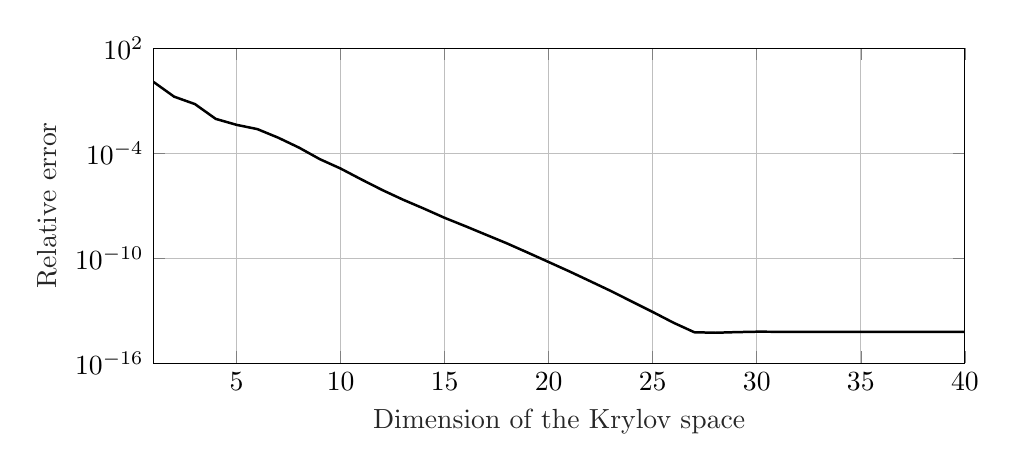
\begin{tikzpicture}

\begin{axis}[%
width=.85\linewidth,
height=4cm,
at={(0in,0in)},
scale only axis,
xmin=1,
xmax=40,
xlabel style={font=\color{white!15!black}},
xlabel={Dimension of the Krylov space},
ymode=log,
ymin=1e-16,
ymax=100,
yminorticks=true,
ylabel style={font=\color{white!15!black}},
ylabel={Relative error},
axis background/.style={fill=white},
xmajorgrids,
ymajorgrids,
yminorgrids,
legend style={legend cell align=left, align=left, draw=white!15!black}
]
\addplot [color=black, line width=0.9pt]
  table[row sep=crcr]{%
1	1.1970666841712\\
2	0.169080928746973\\
3	0.0636940730507964\\
4	0.00908042059055621\\
5	0.00414871323651826\\
6	0.00236609497417638\\
7	0.000766896348482475\\
8	0.000207499206291239\\
9	4.5468096002382e-05\\
10	1.3189262330513e-05\\
11	3.14525985651137e-06\\
12	7.83654425173314e-07\\
13	2.19404091753492e-07\\
14	6.80556241974471e-08\\
15	2.00761703179977e-08\\
16	6.68924820811396e-09\\
17	2.14505152308309e-09\\
18	6.93255504657795e-10\\
19	2.05483068858047e-10\\
20	5.98199450964638e-11\\
21	1.73494311883148e-11\\
22	4.77956305951699e-12\\
23	1.30520399685991e-12\\
24	3.28540461009388e-13\\
25	8.38065195569727e-14\\
26	2.03158589692223e-14\\
27	5.81332239277395e-15\\
28	5.44489077592386e-15\\
29	5.8980465774604e-15\\
30	6.23518964189752e-15\\
31	6.19390114291783e-15\\
32	6.11805363564131e-15\\
33	6.09205637160788e-15\\
34	6.14371904504169e-15\\
35	6.17541894368464e-15\\
36	6.12644428023124e-15\\
37	6.09499001710448e-15\\
38	6.1465375480684e-15\\
39	6.11087985201717e-15\\
40	6.12885950388518e-15\\
};
%\addlegendentry{data1}

\end{axis}
\end{tikzpicture}%
        \caption{}
        \label{fig:ode_conv}
    \end{subfigure}\hspace{.05\linewidth}
    \begin{subfigure}[b]{.45\linewidth}
        \input{figures/ode_sparse.tex}
        \caption{}
        \label{fig:ose_sparse}
    \end{subfigure}
    \caption{Convergence of our algorithm for computing $f(\mathbf{A})\mathbf{b}$ for solving the ODE (equation \ref{eq:odesolution}). We note that on our setup, $\mathbf{A}\in\mathbb{C}^{2500\times 2500}$. Machine precision is quickly reached, at only dimension 27 (a). The matrix $\mathbf{A}$ is strongly structured (b).}
    \label{fig:ode_comp}
\end{figure}

Interestingly, we note that the choice of parameters in the ODE is having a big impact on the performance of the algorithm. If we vary the diffusivity $\epsilon$, we observe that the convergence is considerably slowed down (figure \ref{fig:ode_eps}). The algorithm remains quicker than the naive approach, though it seems important to bear in mind that minor perturbation to some of the problem's component (figures \ref{fig:ode_0.05} and \ref{fig:ode_0.1}) can lead to a considerable change in the convergence behavior.

\begin{figure}
    \begin{subfigure}[b]{.45\linewidth}
        % This file was created by matlab2tikz.
%
%The latest updates can be retrieved from
%  http://www.mathworks.com/matlabcentral/fileexchange/22022-matlab2tikz-matlab2tikz
%where you can also make suggestions and rate matlab2tikz.
%
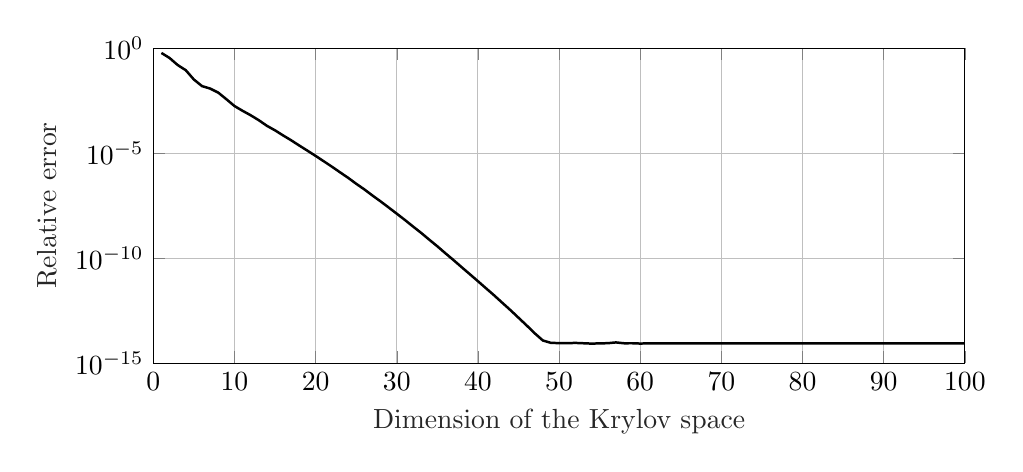
\begin{tikzpicture}

\begin{axis}[%
width=.85\linewidth,
height=4cm,
at={(0in,0in)},
scale only axis,
xmin=0,
xmax=100,
xlabel style={font=\color{white!15!black}},
xlabel={Dimension of the Krylov space},
ymode=log,
ymin=1e-15,
ymax=1,
yminorticks=true,
ylabel style={font=\color{white!15!black}},
ylabel={Relative error},
axis background/.style={fill=white},
xmajorgrids,
ymajorgrids,
yminorgrids,
legend style={legend cell align=left, align=left, draw=white!15!black}
]
\addplot [color=black, line width=0.9pt]
  table[row sep=crcr]{%
1	0.590797345125722\\
2	0.341234080677329\\
3	0.157272930997486\\
4	0.0891400660775228\\
5	0.0320705757210709\\
6	0.0155937592828873\\
7	0.0119253439510956\\
8	0.00763647480225516\\
9	0.00370976324235097\\
10	0.00175449739195379\\
11	0.00103882739089212\\
12	0.000637211140479853\\
13	0.000369644822326709\\
14	0.00020025589215471\\
15	0.00012171128732808\\
16	6.94790567940788e-05\\
17	4.06274966953835e-05\\
18	2.28586221106122e-05\\
19	1.30573267555829e-05\\
20	7.38475979640541e-06\\
21	4.11777447737777e-06\\
22	2.2746904704151e-06\\
23	1.22834302529417e-06\\
24	6.71482740589636e-07\\
25	3.48130942832957e-07\\
26	1.882948292104e-07\\
27	9.62426101173857e-08\\
28	5.06505526015461e-08\\
29	2.58114340082748e-08\\
30	1.30835245506393e-08\\
31	6.57910223892581e-09\\
32	3.21453549599977e-09\\
33	1.59798125349195e-09\\
34	7.57153668307443e-10\\
35	3.66232192610335e-10\\
36	1.69377073233484e-10\\
37	8.01276854328485e-11\\
38	3.69522134517387e-11\\
39	1.72010932723169e-11\\
40	7.96657519147638e-12\\
41	3.65648730747314e-12\\
42	1.68429788109203e-12\\
43	7.48545090813516e-13\\
44	3.35657977698355e-13\\
45	1.44881706755593e-13\\
46	6.25334721934521e-14\\
47	2.63123292955714e-14\\
48	1.1960413249196e-14\\
49	9.20990245321545e-15\\
50	8.98273327994632e-15\\
51	8.90970086473988e-15\\
52	9.16748574882774e-15\\
53	8.82775960859607e-15\\
54	8.49899888132768e-15\\
55	8.70717663222432e-15\\
56	8.89523017820352e-15\\
57	9.6665709467992e-15\\
58	8.82244157379507e-15\\
59	8.84036448276274e-15\\
60	8.54206663471901e-15\\
61	8.73570110668757e-15\\
62	8.73570110668757e-15\\
63	8.73570110668757e-15\\
64	8.73570110668757e-15\\
65	8.73570110668757e-15\\
66	8.73570110668757e-15\\
67	8.73570110668757e-15\\
68	8.73570110668757e-15\\
69	8.73570110668757e-15\\
70	8.73570110668757e-15\\
71	8.73570110668757e-15\\
72	8.73570110668757e-15\\
73	8.73570110668757e-15\\
74	8.73570110668757e-15\\
75	8.73570110668757e-15\\
76	8.73570110668757e-15\\
77	8.73570110668757e-15\\
78	8.73570110668757e-15\\
79	8.73570110668757e-15\\
80	8.73570110668757e-15\\
81	8.73570110668757e-15\\
82	8.73570110668757e-15\\
83	8.73570110668757e-15\\
84	8.73570110668757e-15\\
85	8.73570110668757e-15\\
86	8.73570110668757e-15\\
87	8.73570110668757e-15\\
88	8.73570110668757e-15\\
89	8.73570110668757e-15\\
90	8.73570110668757e-15\\
91	8.73570110668757e-15\\
92	8.73570110668757e-15\\
93	8.73570110668757e-15\\
94	8.73570110668757e-15\\
95	8.73570110668757e-15\\
96	8.73570110668757e-15\\
97	8.73570110668757e-15\\
98	8.73570110668757e-15\\
99	8.73570110668757e-15\\
100	8.73570110668757e-15\\
};
%\addlegendentry{data1}

\end{axis}
\end{tikzpicture}%
        \caption{$\epsilon = 0.05$}
        \label{fig:ode_0.05}
    \end{subfigure}\hspace{.05\linewidth}
    \begin{subfigure}[b]{.45\linewidth}
        % This file was created by matlab2tikz.
%
%The latest updates can be retrieved from
%  http://www.mathworks.com/matlabcentral/fileexchange/22022-matlab2tikz-matlab2tikz
%where you can also make suggestions and rate matlab2tikz.
%
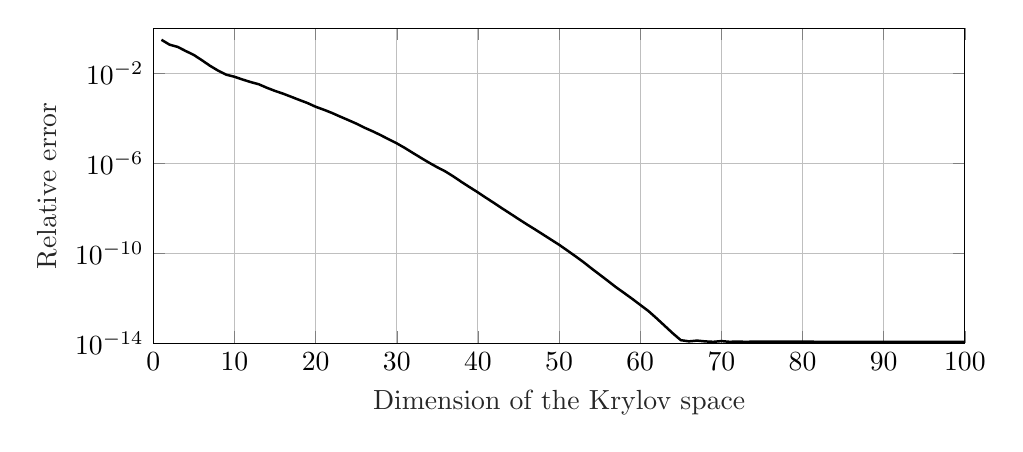
\begin{tikzpicture}

\begin{axis}[%
width=.85\linewidth,
height=4cm,
at={(0in,0in)},
scale only axis,
xmin=0,
xmax=100,
xlabel style={font=\color{white!15!black}},
xlabel={Dimension of the Krylov space},
ymode=log,
ymin=1e-14,
ymax=1,
yminorticks=true,
ylabel style={font=\color{white!15!black}},
ylabel={Relative error},
axis background/.style={fill=white},
xmajorgrids,
ymajorgrids,
yminorgrids,
legend style={legend cell align=left, align=left, draw=white!15!black}
]
\addplot [color=black, line width=0.9pt]
  table[row sep=crcr]{%
1	0.305908729770176\\
2	0.185842348482017\\
3	0.148004926114265\\
4	0.0967602920715717\\
5	0.0648025410697794\\
6	0.0374906795616609\\
7	0.0212681986876963\\
8	0.0129404303440192\\
9	0.00857636695438943\\
10	0.00696983122246\\
11	0.0052436702771879\\
12	0.0040430520213184\\
13	0.00322793629662881\\
14	0.00225043739467314\\
15	0.00163420989998425\\
16	0.0012317053085581\\
17	0.000894599827770048\\
18	0.000646481190339189\\
19	0.000472641931763846\\
20	0.000323747503937065\\
21	0.000239237232699965\\
22	0.000172464606407331\\
23	0.000119267767777074\\
24	8.33546869160878e-05\\
25	5.79065746368e-05\\
26	3.83310896870106e-05\\
27	2.64973950305888e-05\\
28	1.77956353172652e-05\\
29	1.1572385222042e-05\\
30	7.63111644290351e-06\\
31	4.75642097235582e-06\\
32	2.84007682669571e-06\\
33	1.71696918621979e-06\\
34	1.04443317998124e-06\\
35	6.57734489776193e-07\\
36	4.28651820530108e-07\\
37	2.55066150563038e-07\\
38	1.45231230007161e-07\\
39	8.52079339309969e-08\\
40	5.04567246510479e-08\\
41	2.90386860768354e-08\\
42	1.69052039752362e-08\\
43	9.73916094512884e-09\\
44	5.70287754878932e-09\\
45	3.31176300104464e-09\\
46	1.94267818061846e-09\\
47	1.16221732506671e-09\\
48	6.86205349497406e-10\\
49	4.0331986801663e-10\\
50	2.3777682784408e-10\\
51	1.33195796008228e-10\\
52	7.38789284933916e-11\\
53	4.03691572879177e-11\\
54	2.09532560448374e-11\\
55	1.11688818330872e-11\\
56	5.9290452312746e-12\\
57	3.10778224572015e-12\\
58	1.72293872958609e-12\\
59	9.430732382795e-13\\
60	5.05177562527383e-13\\
61	2.70453670846753e-13\\
62	1.29267808561687e-13\\
63	5.99638388081284e-14\\
64	2.77124868607469e-14\\
65	1.36416588675984e-14\\
66	1.20608922532971e-14\\
67	1.30538908154694e-14\\
68	1.20204110642728e-14\\
69	1.15053833173926e-14\\
70	1.23939147588686e-14\\
71	1.15288488594861e-14\\
72	1.17708949199402e-14\\
73	1.15099822915781e-14\\
74	1.17115726182429e-14\\
75	1.16095322259592e-14\\
76	1.17422209767356e-14\\
77	1.18564037625219e-14\\
78	1.16831660905169e-14\\
79	1.18867501777877e-14\\
80	1.17585807800807e-14\\
81	1.1734565908154e-14\\
82	1.14063627929465e-14\\
83	1.14063627929465e-14\\
84	1.14063627929465e-14\\
85	1.14063627929465e-14\\
86	1.14063627929465e-14\\
87	1.14063627929465e-14\\
88	1.14063627929465e-14\\
89	1.14063627929465e-14\\
90	1.14063627929465e-14\\
91	1.14063627929465e-14\\
92	1.14063627929465e-14\\
93	1.14063627929465e-14\\
94	1.14063627929465e-14\\
95	1.14063627929465e-14\\
96	1.14063627929465e-14\\
97	1.14063627929465e-14\\
98	1.14063627929465e-14\\
99	1.14063627929465e-14\\
100	1.14063627929465e-14\\
};
%\addlegendentry{data1}

\end{axis}
\end{tikzpicture}%
        \caption{$\epsilon = 0.1$}
        \label{fig:ode_0.1}
    \end{subfigure}
    \caption{Convergence of our algorithm for different diffusivity value $\epsilon$. We note that as the dissufivity increases, the need to work in higher dimension increases too, thus slowing down the convergence of our algorithm. }
    \label{fig:ode_eps}
\end{figure}

\subsection{The sign function}
In control theory we are often interested in the eigenvalues $\lambda$ of system matrices with $Re(\lambda)>0$, since they correspond to unstable poles. In the design of controllers it is therefore interesting to have an efficient way to count the number of eigenvalues of a matrix in the right half-plane $Re(z)>0$. Here we will build such a method.
\begin{theorem}\label{thm:sign}
Let $\mathbf{A}\in\mathbb{C}^{n \times n}$ be a matrix with $k_{-}$ eigenvalues in the left plane, $k_{+}$ eigenvalues in the right plane and none on the imaginary axis, counting multiplicity. Let $\text{sgn}:\mathbb{C}\mapsto \{1,-1\}$ be defined by
$$\text{sgn}(z)= \begin{cases} 
      1 & Re(z)\geq 0 \\
      -1 & Re(z)<0. 
   \end{cases}
$$
Then $\text{trace}(\text{sgn}(\mathbf{A}))=k_{+}-k_{-}$.
\end{theorem}
\begin{proof}
    Let $\mathbf{A}\in\mathbb{C}^{n\times n}$. To stay in a very general scenario, and consider cases where $\mathbf{A}$, let us consider its Jordan Canonical Form :
    \begin{equation*}
        \mathbf{A} = \mathbf{VJV}^{-1}
    \end{equation*} 
    Recall that by theorem \ref{thm:jordan}, consider $f$ a function, then 
    \begin{equation*}
        f(\mathbf{A}) = \mathbf{V}f(\mathbf{J})\mathbf{V}^{-1}
    \end{equation*}
    Thus let us consider the decomposition where 
    \begin{equation*}
        \mathbf{J} = \begin{pmatrix}
            \mathbf{J}_{k_+} & 0 \\ 0 & \mathbf{J}_{k_-}
        \end{pmatrix}
    \end{equation*}
    such that $\mathbf{J}_{k_+}$ has $k_+$ eigenvalues in the right plane, and $\mathbf{J}_{k_-}$ has $k_-$ eigenvalues in the left plane. Then, we have that
    \begin{equation*}
        \text{sgn}(\mathbf{J}) = \begin{pmatrix}
            \mathbf{I}_{k_+} & 0 \\ 0 & -\mathbf{I}_{k_-}
        \end{pmatrix}
    \end{equation*}
    where $\mathbf{I}_n$ is the identity matrix of size $n$. Then, we have that
    \begin{equation*}
        \text{trace}(\text{sgn}(\mathbf{J})) = k_+ - k_-
    \end{equation*}
    And thus, we have that
    \begin{equation*}
        \text{trace}(\text{sgn}(\mathbf{A})) = \text{trace}(\text{sgn}(\mathbf{VJV}^{-1})) = \mathbf{V}\text{trace}(\text{sgn}(\mathbf{J}))\mathbf{V}^{-1} = (k_+-k_-)\mathbf{V}\mathbf{V}^{-1} = k_+ - k_-
    \end{equation*}
\end{proof}
\printbibliography
\end{document}